%-------------------------------------------------------------------------------
% RESULTS AND DISCUSSION
%-------------------------------------------------------------------------------

\section{Results and Discussion} \label{sec:resdisc}

The primary objective is to reproduce the bifurcation diagram presented in
Figure \ref{fig:bif_diag_chen} of \citet{chen2013}. The bifurcation diagram of
the regularized version is depicted below (figure \ref{fig:bif_diag}), and a
table is provided, listing the bifurcations that occurred along with their
corresponding critical Reynolds numbers. As mentioned, only a square cavity is
considered for this study, and no aspect ratios have been varied. But this can
easily be done by using two differentiation matrices, which is explained in
section \ref{sec:2d_cheb}.

The critical Reynolds numbers reported were determined by linearly
interpolating the eigenvalues between two states of the pseudo-arclength
continuation algorithm where the eigenvalue crosses the imaginary axis in the
complex plane. When eigenvalues are only touching the real line (i.e. no
crossing), the Reynolds number with the smallest eigenvalue evaluated has been
reported.

\begin{table}[h!]
  \centering
  \caption{List of bifurcations encountered and the critical $\Rey$ at which they
    occur}
  \label{tab:bif_points}
\begin{tabular}{l c}
Bifurcation & $\Rey$\\
\hline
$P_1$, first super-critical pitchfork of the base flow & $66.197$ \\
$P_2$, second pitchfork of the base flow & $172.708$ \\
$P_3$, third pitchfork of asymmetric steady solution close to saddle-node & $353.357$ \\
$SN$, saddle-node bifurcation of the asymmetric steady solution & $353.654$ \\
$H$, Hopf bifurcation of the asymmetric steady solution & $348.319$ \\
\end{tabular}
\end{table}

\begin{table}[h!]
  \centering
  \caption{Critical Reynolds numbers depending on the grid size $m$ of the two
    pitchfork bifurcations of the symmetric base flow, $\Rey_c^{P_1}$ and
    $\Rey_c^{P_2}$, and of the saddle-node, the third pitchfork and Hopf
    bifurcations corresponding to the asymmetric steady solution,
    $\Rey_c^{SN}$, $\Rey_c^{P_3}$ and $\Rey_c^{H}$ respectively. For the Hopf
    bifurcation, the imaginary part $\omega_c^{H}$ corresponding to the crossing
    eigenvalue has also been included. In comparison, the critical values for the
    un-regularized version are shown as well.}
  \label{tab:re_crit}
\begin{tabular}{crrrrrr}
$m$ & $\Rey_c^{P_1}$ & $\Rey_c^{P_2}$ & $\Rey_c^{H}$ &  $\omega_c^{H}$ & $\Rey_c^{P_3}$ & $\Rey_c^{SN}$  \\
\hline
$32$ & $66.197$ & $172.731$ & $348.210$ & $0.0582$ & $352.152$ & $352.527$ \\
$48$ & $66.197$ & $172.708$ & $348.312$ & $0.0588$ & $353.365$ & $353.663$ \\
$64$ & $66.197$ & $172.708$ & $348.319$ & $0.0599$ & $353.356$ & $353.656$ \\
$96$ & $66.197$ & $172.708$ & $348.319$ & $0.0599$ & $353.357$ & $353.654$ \\
\citet{chen2013} & $65.154$ & $177.723$ & - $\quad$ & - $\quad$ & - $\quad$ & $438.285$ \\
\end{tabular}
\end{table}

\begin{figure}[h!]
  \centering
  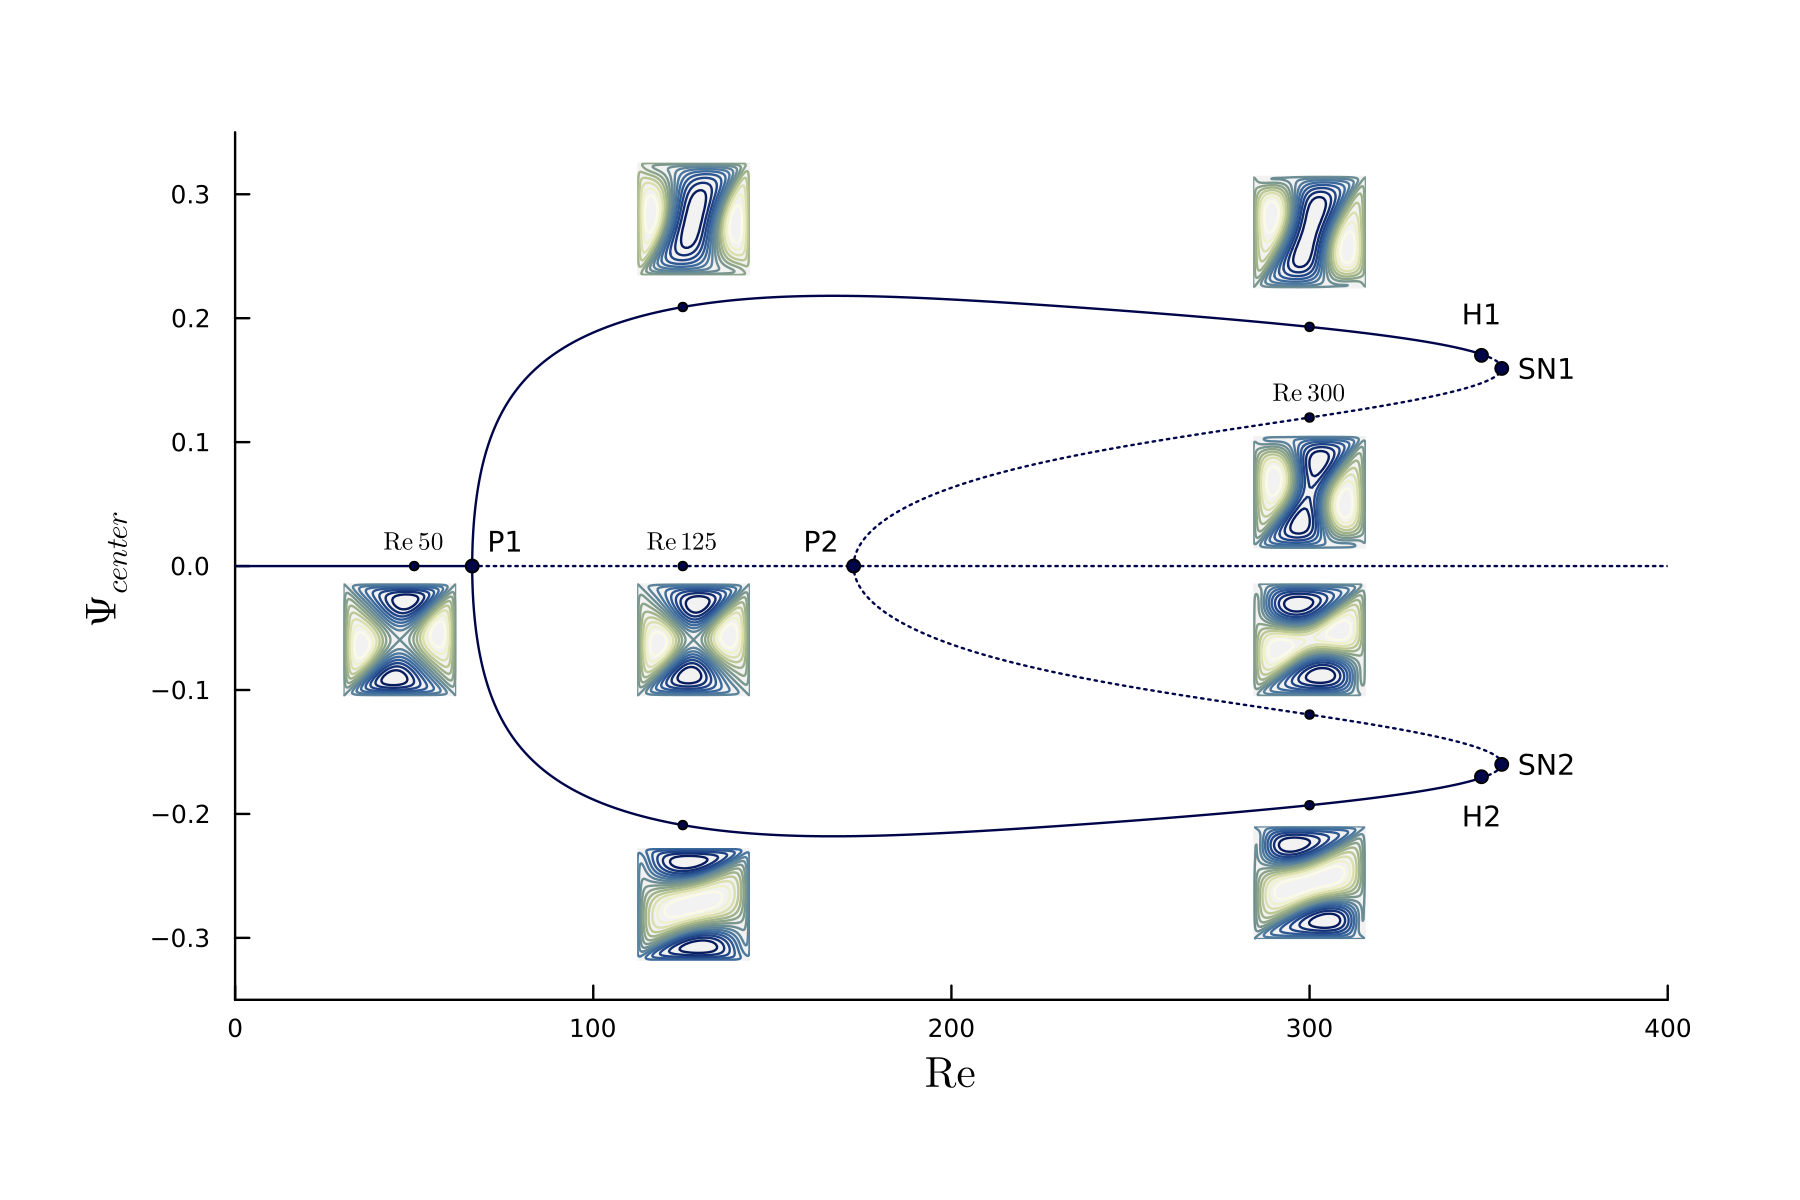
\includegraphics[width=\textwidth]{figs/bifurcation_diag64x64.png}
  \caption{Bifurcation diagram for the regularized version of the four-sided
    cavity flow, calculated with the developed Julia module} 
  \label{fig:bif_diag}
\end{figure}

Analyzing the new bifurcation diagram in figure \ref{fig:bif_diag} shows that
the regularized version resembles the non-regularized one regarding
bifurcations and the shape of the asymmetric branches. The reported critical
Reynolds numbers for the pitchforks $P_1$ and $P_2$ are close to those of the
original problem (scaled by $2$, see section \ref{sec:scale}). We can also see
how the regularized version converges rapidly, with only the third decimal
digits changing from a grid of size $48 \times 48$ or larger for the two
pitchforks and the saddle-node bifurcation. However, it is worth mentioning
that the pitchfork $P_2$ is not a true pitchfork as only unstable branches
(represented by the dashed line) join at this bifurcation.

On the other hand, it has been observed that the critical value for the saddle
node in the regularized version deviates significantly from the original value
by approximately $80$ in Reynolds. However, by increasing the control parameter
$k_0$ (fixed to $10$ in this study), the saddle-node appears to shift further
to the right. Consequently, this adjustment brings it closer to the original
bifurcation point, as it better approximates the discontinuous step function of
the boundary conditions. But on can not expect good results when taking this
limit as the boundary conditions are again "almost" discontinuous.

Moreover, the Group of Nonlinear Fluid Dynamics at UPC discovered a Hopf
bifurcation ($H$) with a critical Reynolds number close to the saddle-node.
This finding has not been reported in any of the previous studies. The question
that arises is if the Hopf bifurcation is super-critical or sub-critical.
Launching a time-stepper with random values of the order of $10^{-3}$ reveals
trajectories converging to stable periodic orbits, shown in figure
\ref{fig:orbit}. In order to visualize the orbit in the phase space and due to
the asymmetry of the solutions, the average of the vertical and horizontal
velocities at the top and left mid-points of the cavity (as depicted in Figure
\ref{fig:cav_domain}) was used. In figure \ref{fig:orbit_bif_diag}, the amplitude of
these oscillations is shown in terms of the center value of the streamfunction
and compared to the unstable branches. Notably, the magnitudes are greater than
the expected square root growth of amplitude for oscillations that characterize
a super-critical Hopf bifurcation. One can also recognize that the stable
periodic orbits pass close to all the locally attracting unstable branches.

\begin{figure}[ht]
  \centering
  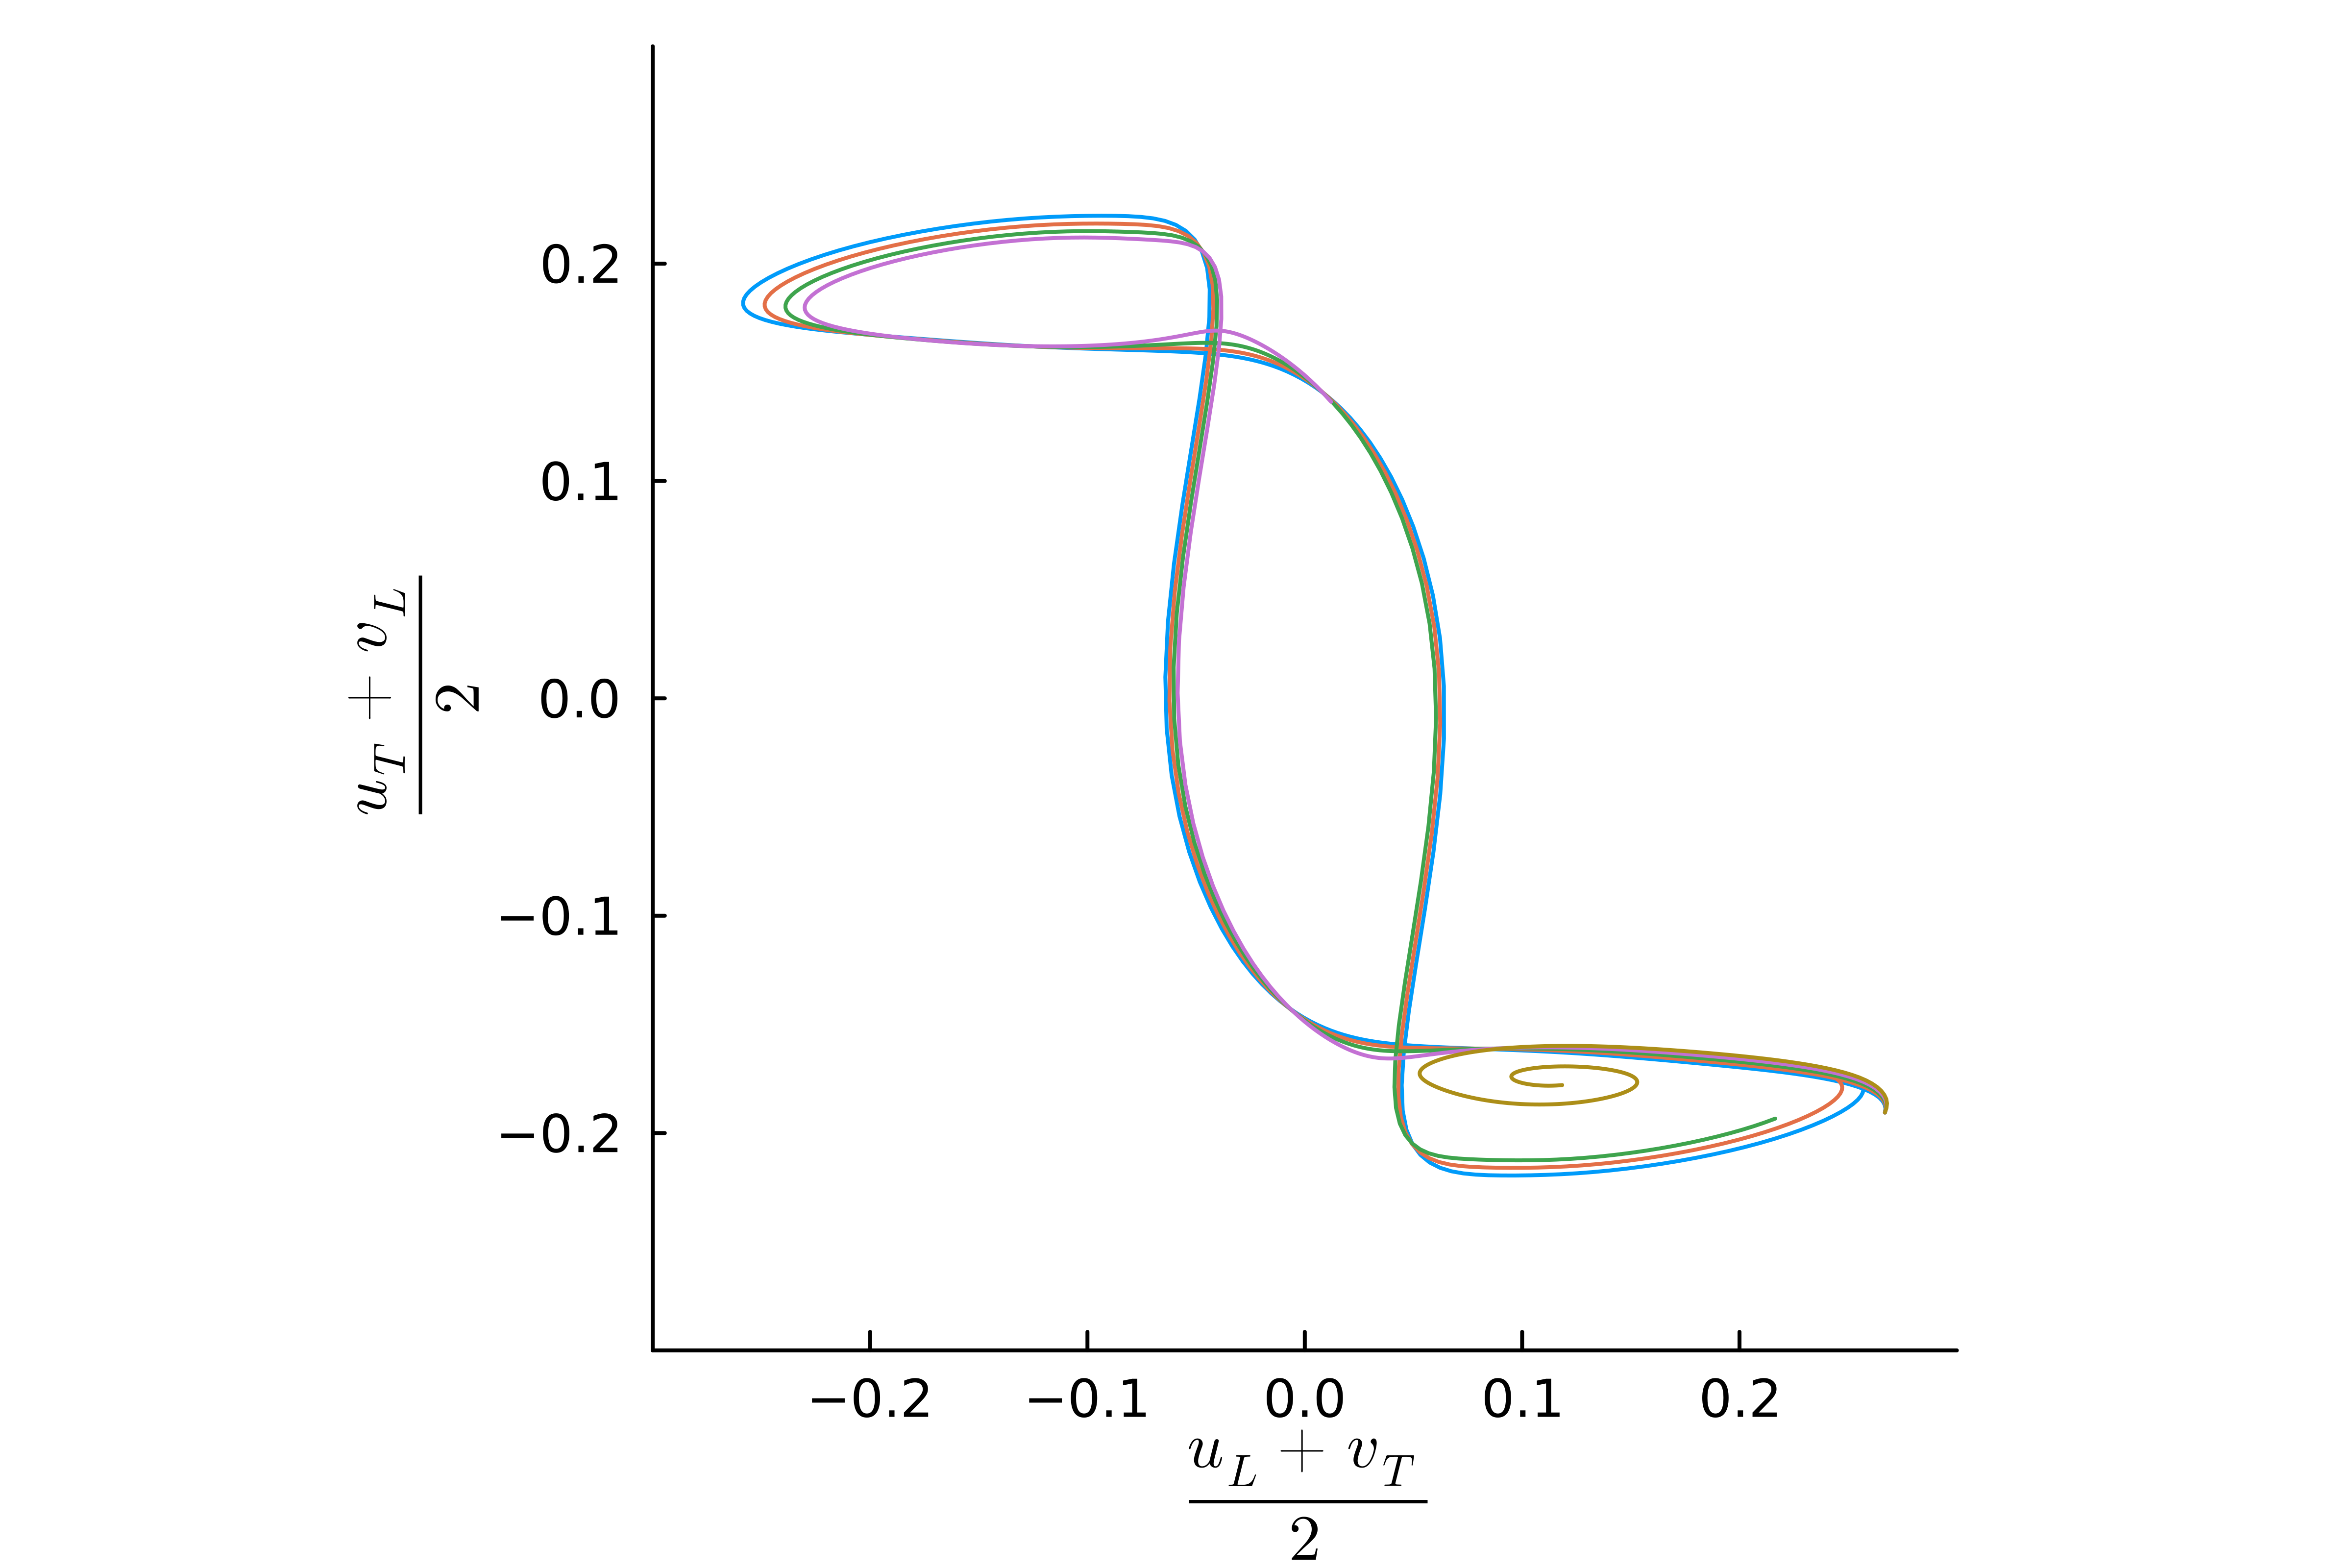
\includegraphics[width=0.65\textwidth]{figs/orbits32x32.png}
  \caption{Periodic orbits at different Reynolds numbers illustrated in phase space (plot not finished).} 
  \label{fig:orbit}
\end{figure}

\begin{figure}[ht]
  \centering
  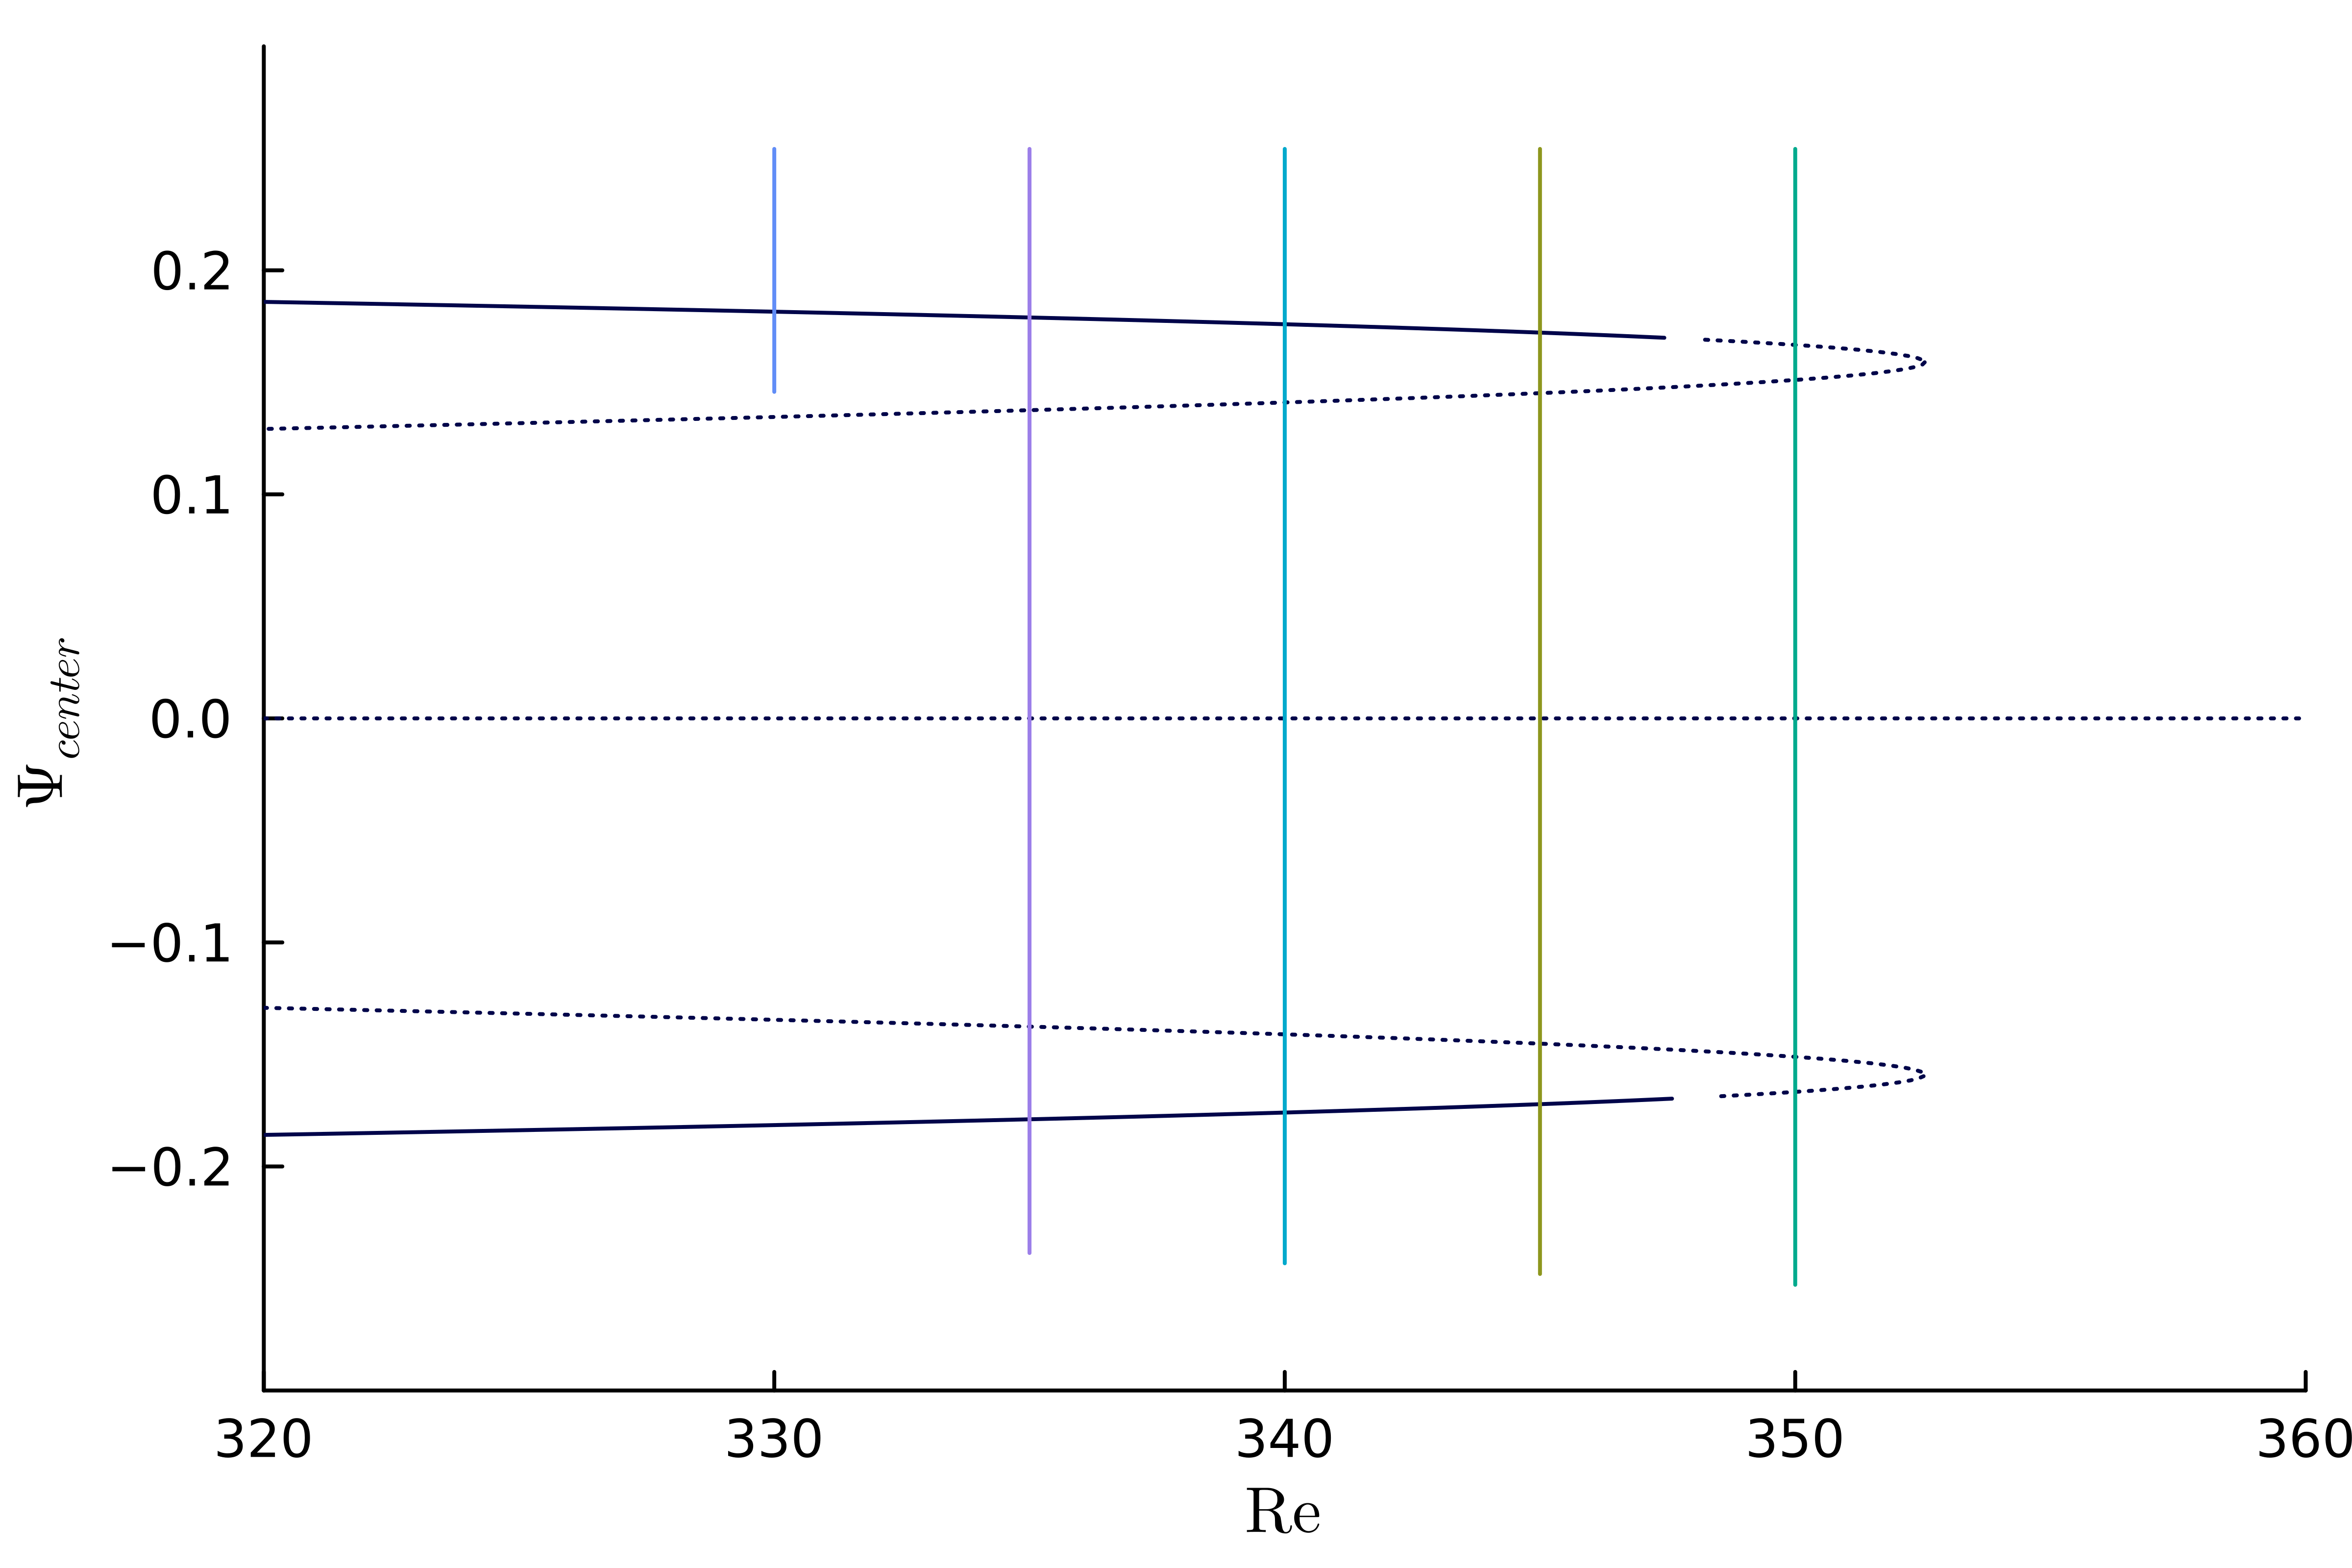
\includegraphics[width=0.6\textwidth]{figs/orbits_bif_diag32x32.png}
  \caption{Center value of streamfunction for the computed periodic orbits of figure \ref{fig:orbit}
  (plot not finished).} 
  \label{fig:orbit_bif_diag}
\end{figure}

It becomes clear that stable orbits exist below the critical Reynolds number of
the Hopf bifurcation. The periodic orbits below this Reynolds number are
obtained by extracting the solutions of the $\Psi$ with the maximum amplitude
and utilizing this as initial conditions for a lower Reynolds number in the
time-stepper. Additionally, unstable periodic orbits have been computed using
the MATLAB version, with the Reynolds number lower than the critical value of
the Hopf. The lower branch of these orbits connects to the lower asymmetric
branch through a homoclinic connection. Figure \ref{fig:sub_hopf_sketch}
illustrates what seems to be happening. A saddle-node of orbits joins the upper
branch with the stable periodic orbits depicted in the previous figure. It
seems very likely that this corresponds to a sub-critical Hopf.

\begin{figure}[ht]
\centering
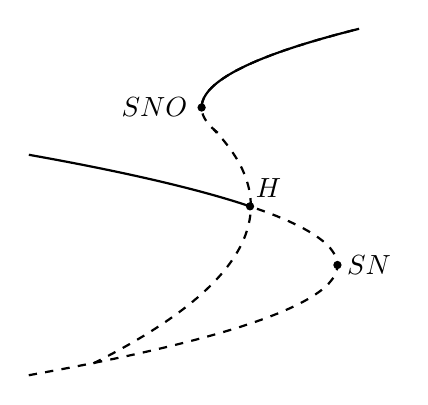
\begin{tikzpicture}[scale=0.5]
  \draw[thick, dashed] plot[smooth,domain=-2.8:1.5] ({-\x*\x},\x);
  \draw[thick] plot[smooth,domain=1.5:2.8] ({-\x*\x},\x);

  \draw[thick, dashed] plot[smooth,domain=-4:1.95] ({-0.25*\x*\x - 2.2},\x + 1.5);

  \draw[thick, dashed] plot[smooth,domain=-0.64:2] ({\x*\x - 3.45},\x + 4);
  \draw[thick] plot[smooth,domain=0:2] ({\x*\x - 3.45},\x + 4);

  \fill (-3.45,4) circle [radius=3pt];
  \fill (-1.49^2,1.49) circle [radius=3pt];
  \fill (0,0) circle [radius=3pt];

  \node at (-1.5^2 + 0.5,1.7 + 0.25) {$H$};
  \node at (-3.45 - 1.2,4) {$SNO$};
  \node at (0.8,0) {$SN$};
\end{tikzpicture}
\caption{Illustration of the saddle-node of orbits ($SNO$) for the potential sub-critical Hopf.} 
\label{fig:sub_hopf_sketch}
\end{figure}

During the linear stability analysis conducted around the saddle-node, another
occurrence of an eigenvalue crossing and gaining a positive real part has been
identified. Figure \ref{fig:lsa} shows the three largest eigenvalues in a plot
where the Reynolds number increases and then decreases again from the
saddle-node onwards. The details of these crossings are presented in table
\ref{tab:cross}. The crossing labeled $A$ corresponds to the complex conjugate
pair associated with the Hopf bifurcation, which is denoted by $\lambda_1$ and
$\lambda_2$ in green. However, another eigenvalue crossing is found just before
the saddle-node, denoted as $B$. This second eigenvalue crossing ($\lambda_3$
in orange) at $B$ occurs in a distance of $0.3$ in Reynolds before to the
saddle-node. \\\\

\begin{minipage}[h]{\textwidth}
\begin{minipage}[b]{.4\textwidth}
\centering
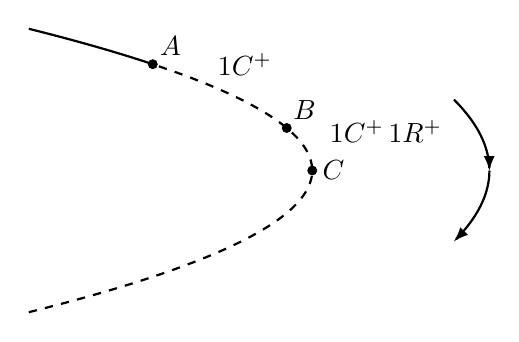
\begin{tikzpicture}[scale=0.9]
  \draw[thick, dashed] plot[smooth,domain=-2:1.5] ({-\x*\x},\x);
  \draw[thick] plot[smooth,domain=1.5:2] ({-\x*\x},\x);

  \draw[-latex, thick] plot[smooth,domain=1:0] ({2.5 + -0.5*\x*\x},\x);
  \draw[-latex, thick] plot[smooth,domain=0:-1] ({2.5 + -0.5*\x*\x},\x);

  \fill (-1.5^2,1.5) circle [radius=2pt];
  \fill (-0.6^2,0.6) circle [radius=2pt];
  \fill (0,0) circle [radius=2pt];

  \node at (-1.5^2 + 0.25,1.5 + 0.25) {$A$};
  \node at (-0.6^2 + 0.25,0.6 + 0.25) {$B$};
  \node at (0.3,0) {$C$};

  \node at (-1.5^2 + 1.3,1.6 - 0.1) {$1\mathbb{C}^{+}$};
  \node at (-0.6^2 + 1.4,0.6 - 0.05) {$1\mathbb{C}^+ \, 1\mathbb{R}^+$};
\end{tikzpicture}
\captionof{figure}{A schematic of the encountered eigenvalue crossing and 
  the direction of the linear stability analysis in figure \ref{fig:lsa}}
\label{fig:schem_saddle}
\end{minipage}\hfill
\begin{minipage}[b]{.4\textwidth}
  \centering
  \begin{tabular}{crrr}
  \label{tab:cross}
  $n$ & $A$ ($H$) & $B$ ($P_3$) & $C$ ($SN$) \\
  \hline
  $64$ & $348.19$ & $353.356$ & $353.656$ \\
  $96$ & $348.19$ & $353.357$ & $353.654$ \\
  & & & \\
  & & & \\
\end{tabular}
\captionof{table}{Critical Reynolds numbers where crossings appear. \newline \newline}
\end{minipage}
\end{minipage}
\smallskip

\begin{figure}[h]
  \centering
  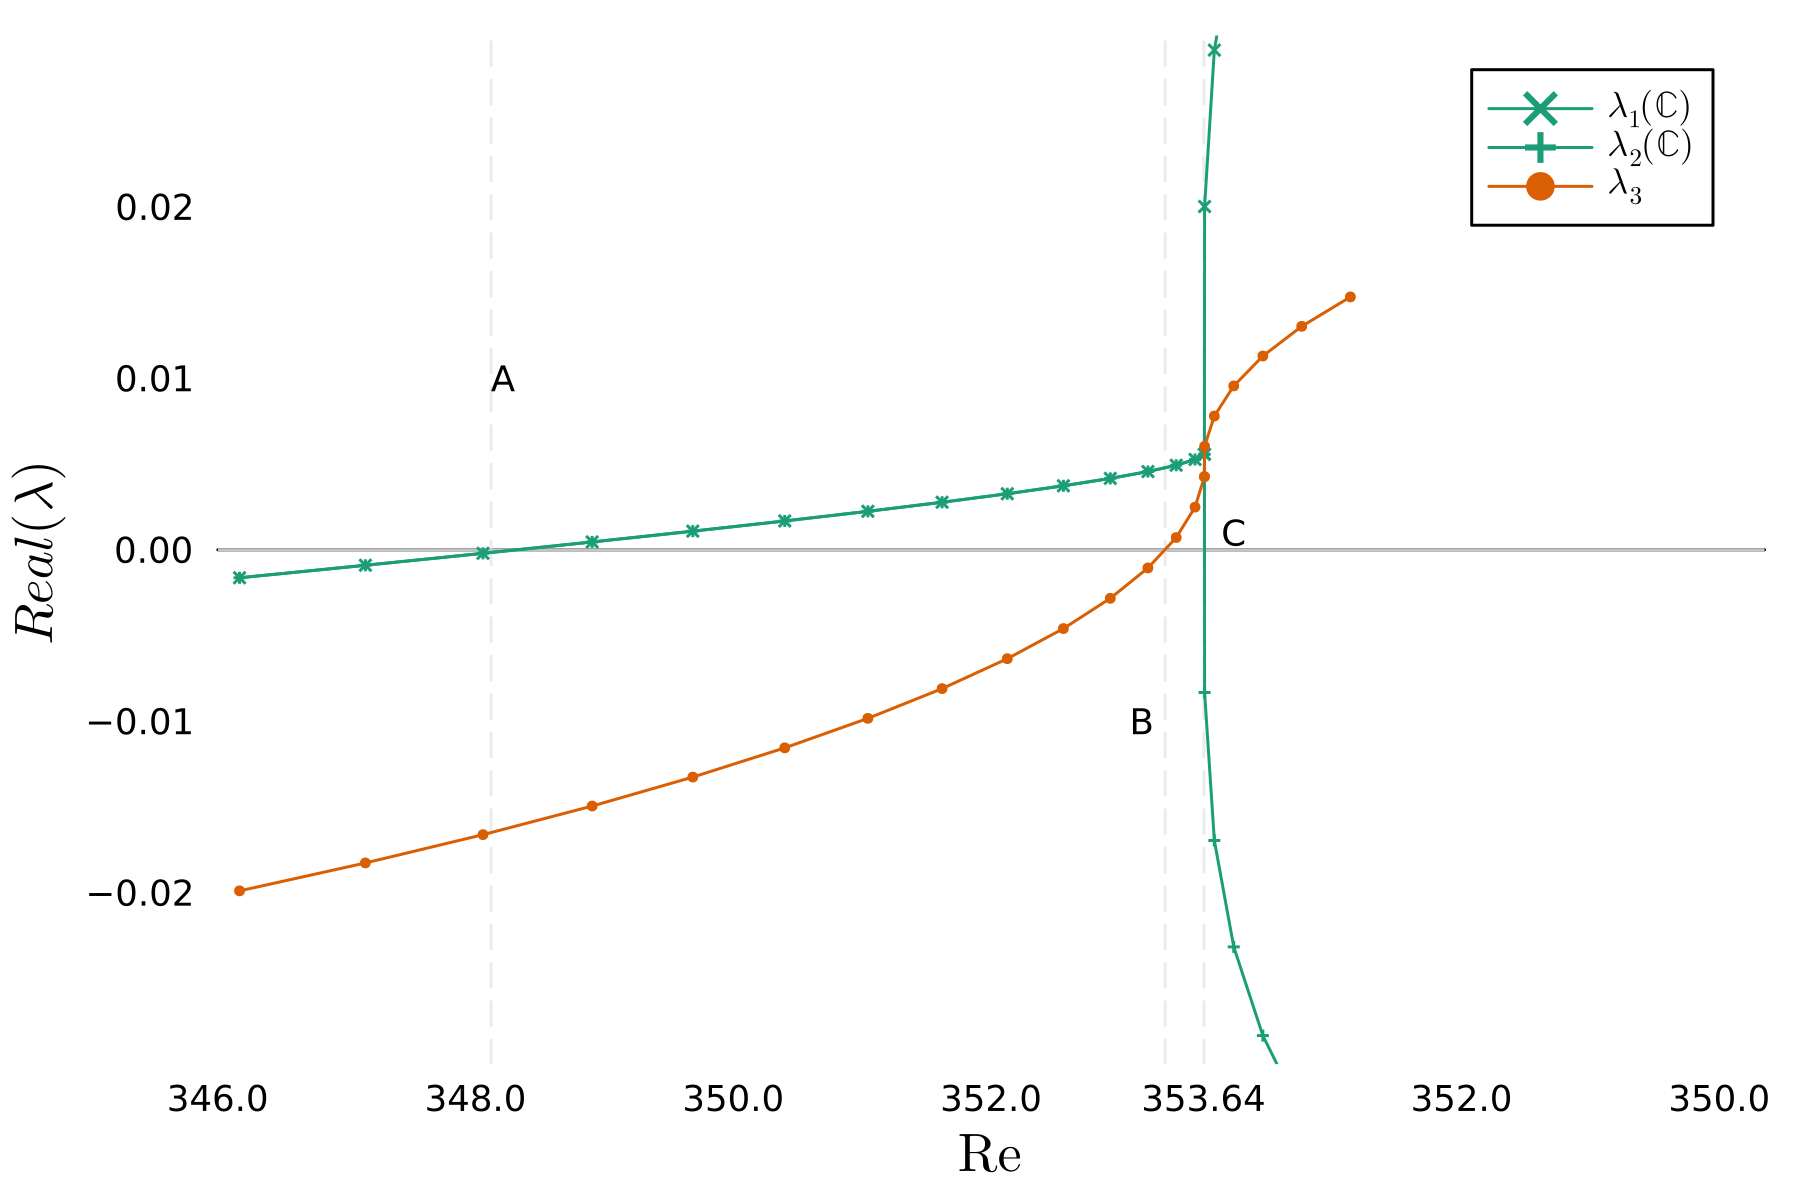
\includegraphics[width=0.8\textwidth]{figs/lsa_sn96x96.png}
  \caption{Linear stability analysis around saddle-node (increasing and
    decreasing Reynolds number). The real part of the three largest eigenvalues
    are shown, grid $96 \times 96$.} 
  \label{fig:lsa}
\end{figure}

Additionally, close to the saddle-node, another unstable branch emerges, and
was detected by starting the natural continuation algorithm near the critical
Reynolds of the fold. This branch is depicted in figure \ref{fig:branch2} and
contains unstable solutions. The figure shows the projections onto the $\Psi$
and $u_T$ planes to distinguish the branches. One can see that for the new
branch, the center value of the streamfunction is not changing significantly,
whereas, for both the asymmetric and the second branch, there is a change in
the value of $u_T$. Further, this branch is connected to point $B$,
corresponding to another pitchfork, denoted by $P_3$. Linear stability analysis
around at the pitchfork of this new branch (figure \ref{fig:lsa_branch2})
reveals how the eigenvalues can be related to point $B$ (i.e. $P_3$). 

\begin{figure}[h!]
  \centering
  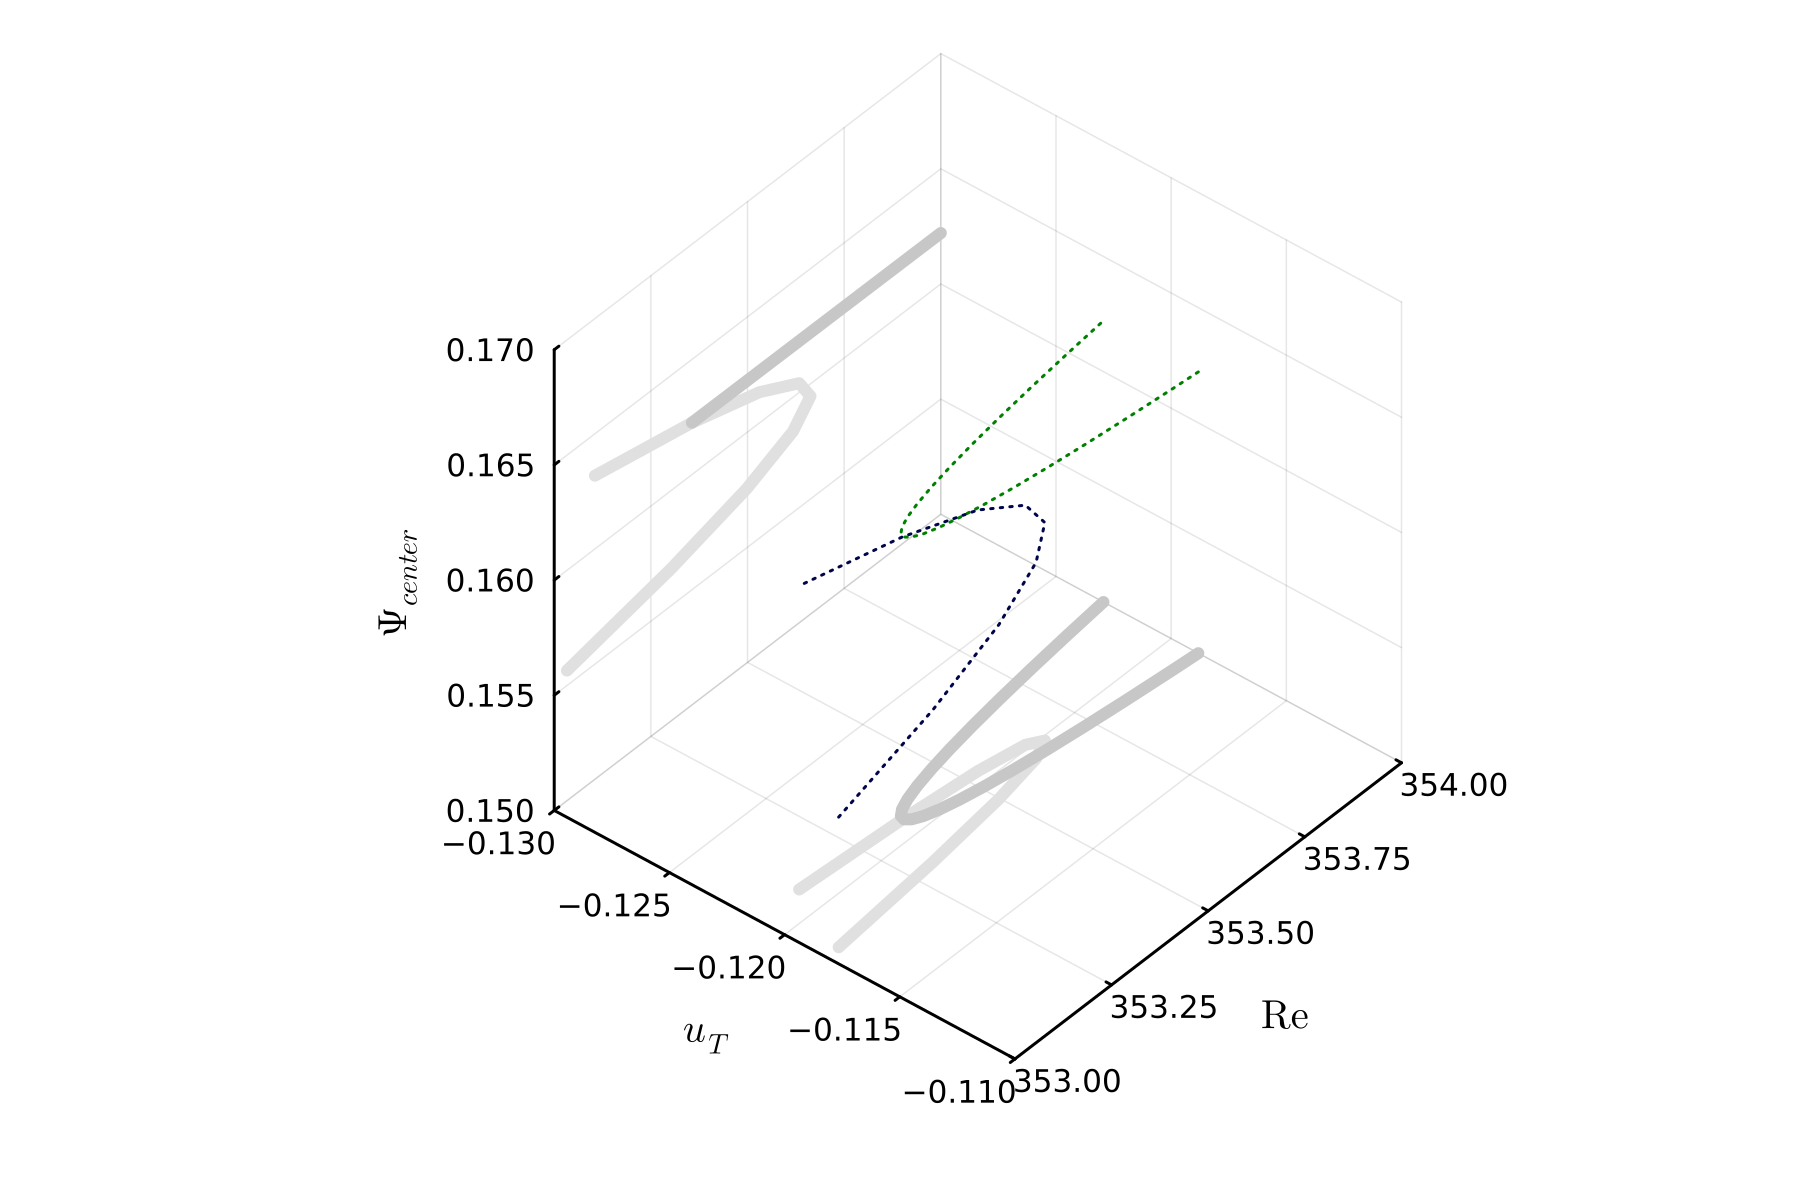
\includegraphics[width=0.9\textwidth]{figs/branch2_64x64.png}
  \caption{3D plot of the asymmetric branch (blue) and second branch (green) and the
    connection of the two branches at point $B$}
  \label{fig:branch2}
\end{figure}

The emergence of the second branch displays another view on the problem. Since
we are dealing with symmetric boundary conditions, we can observe that the
streamlines of the symmetric base solution in the four-sided lid-driven cavity
flow remain unchanged under a $\pi$-rotation of the cavity. The two asymmetric
branches conserve this symmetry as well. Figure \ref{fig:sol_branch2}
illustrates the two solutions of the additional pitchfork emerging at point
$B$, and it can be seen that for these branches, the rotational symmetry is now
also broken. But both branches exhibit a the rotational symmetry with respect
to each other.

\begin{figure}[h!]
\begin{subfigure}[b]{0.33\textwidth}
  \centering
  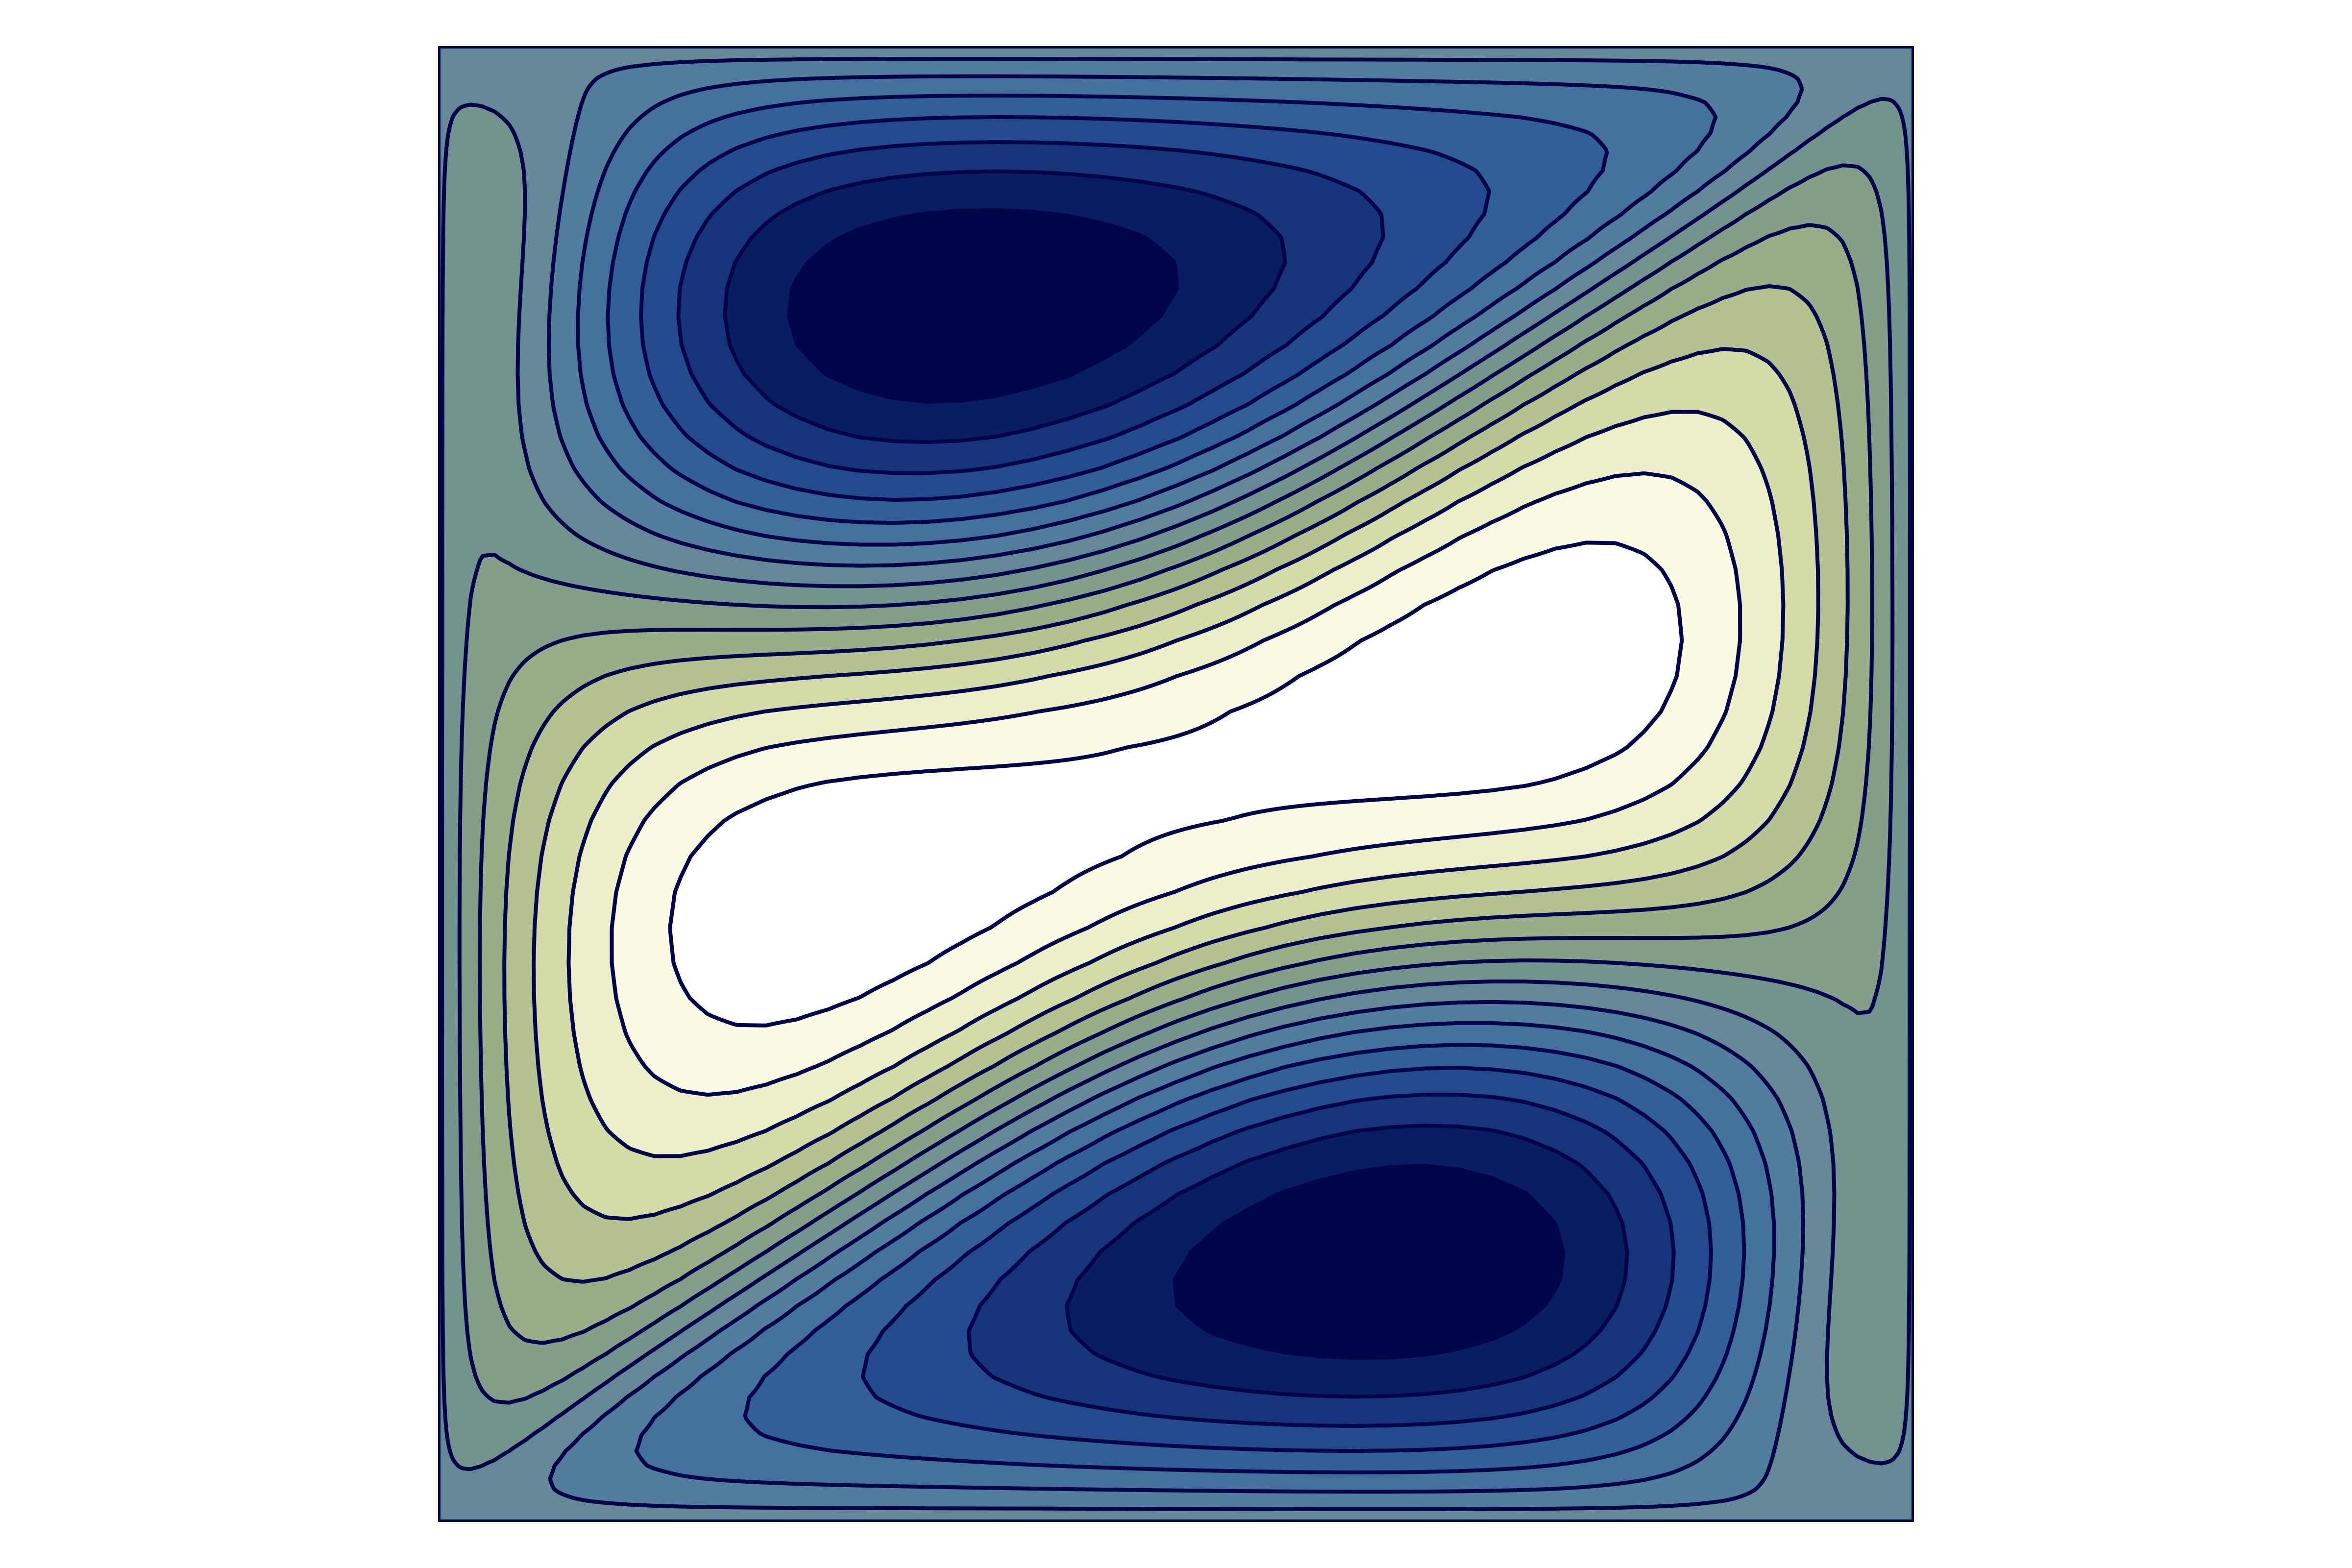
\includegraphics[width=\textwidth]{figs/psi_Re353.356_pf3.png}
\end{subfigure}
\begin{subfigure}[b]{0.33\textwidth}
  \centering
  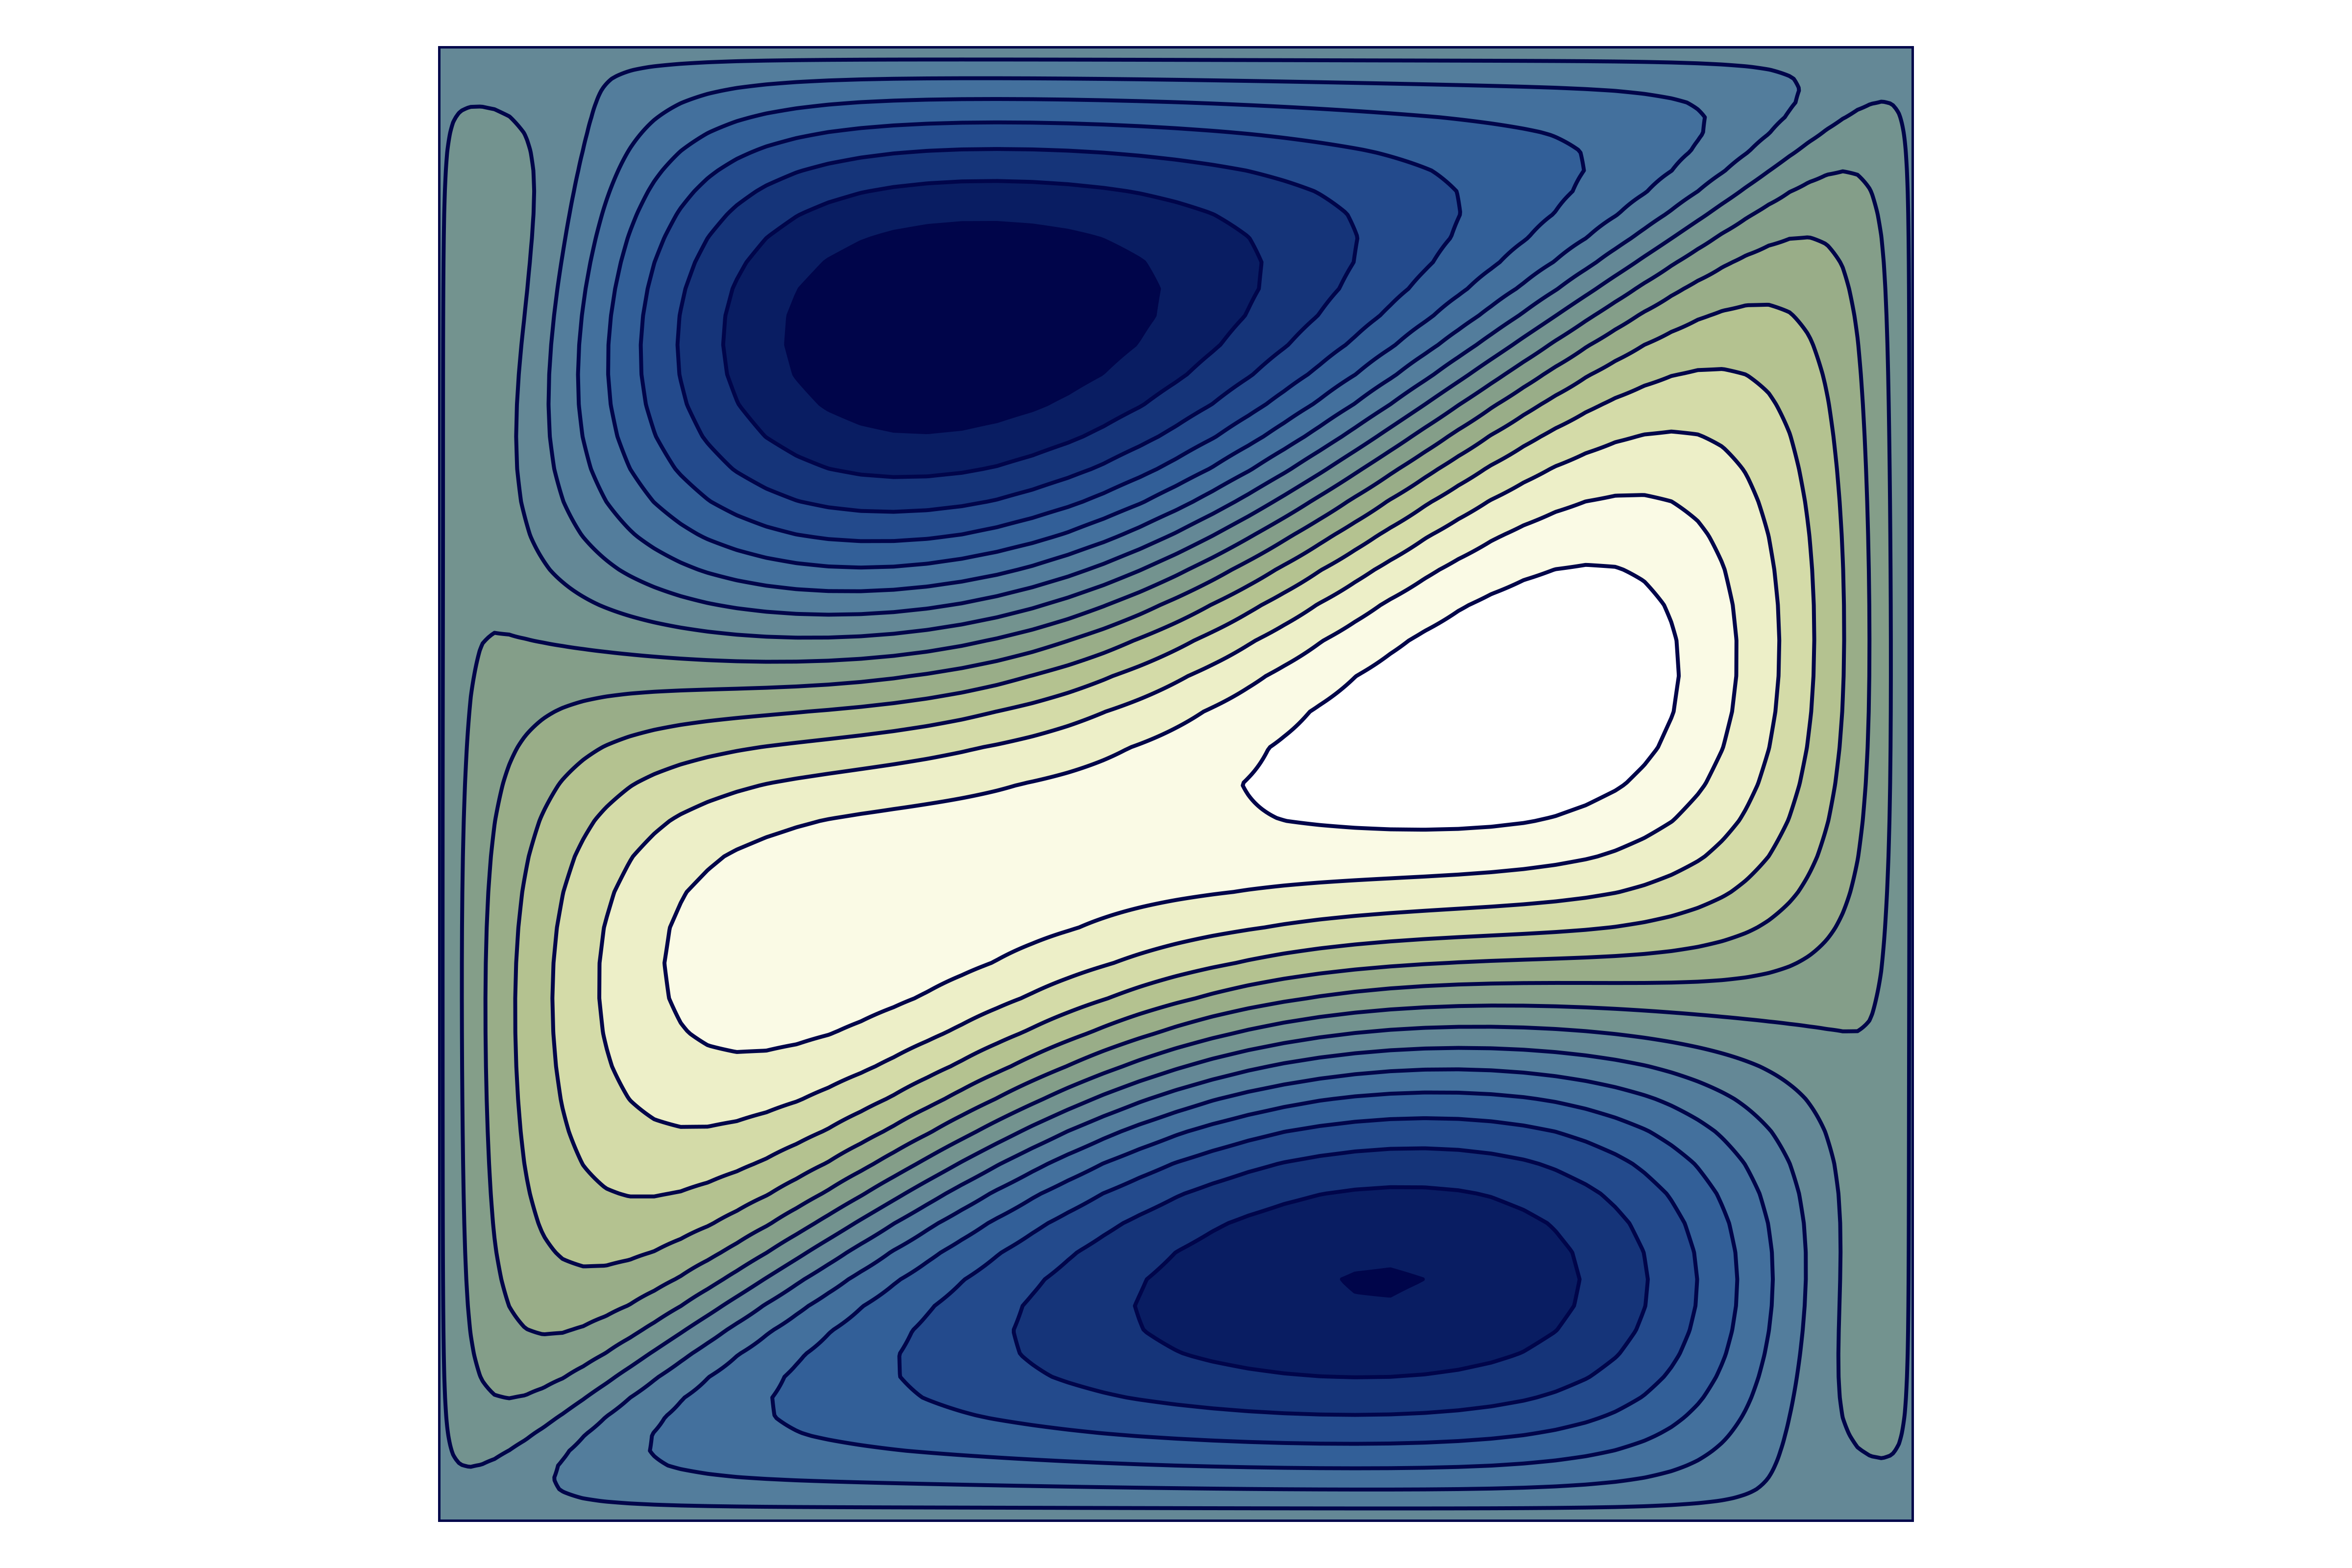
\includegraphics[width=\textwidth]{figs/psi_Re375.000_branch2_u_t_smaller.png}
\end{subfigure}
\begin{subfigure}[b]{0.33\textwidth}
  \centering
  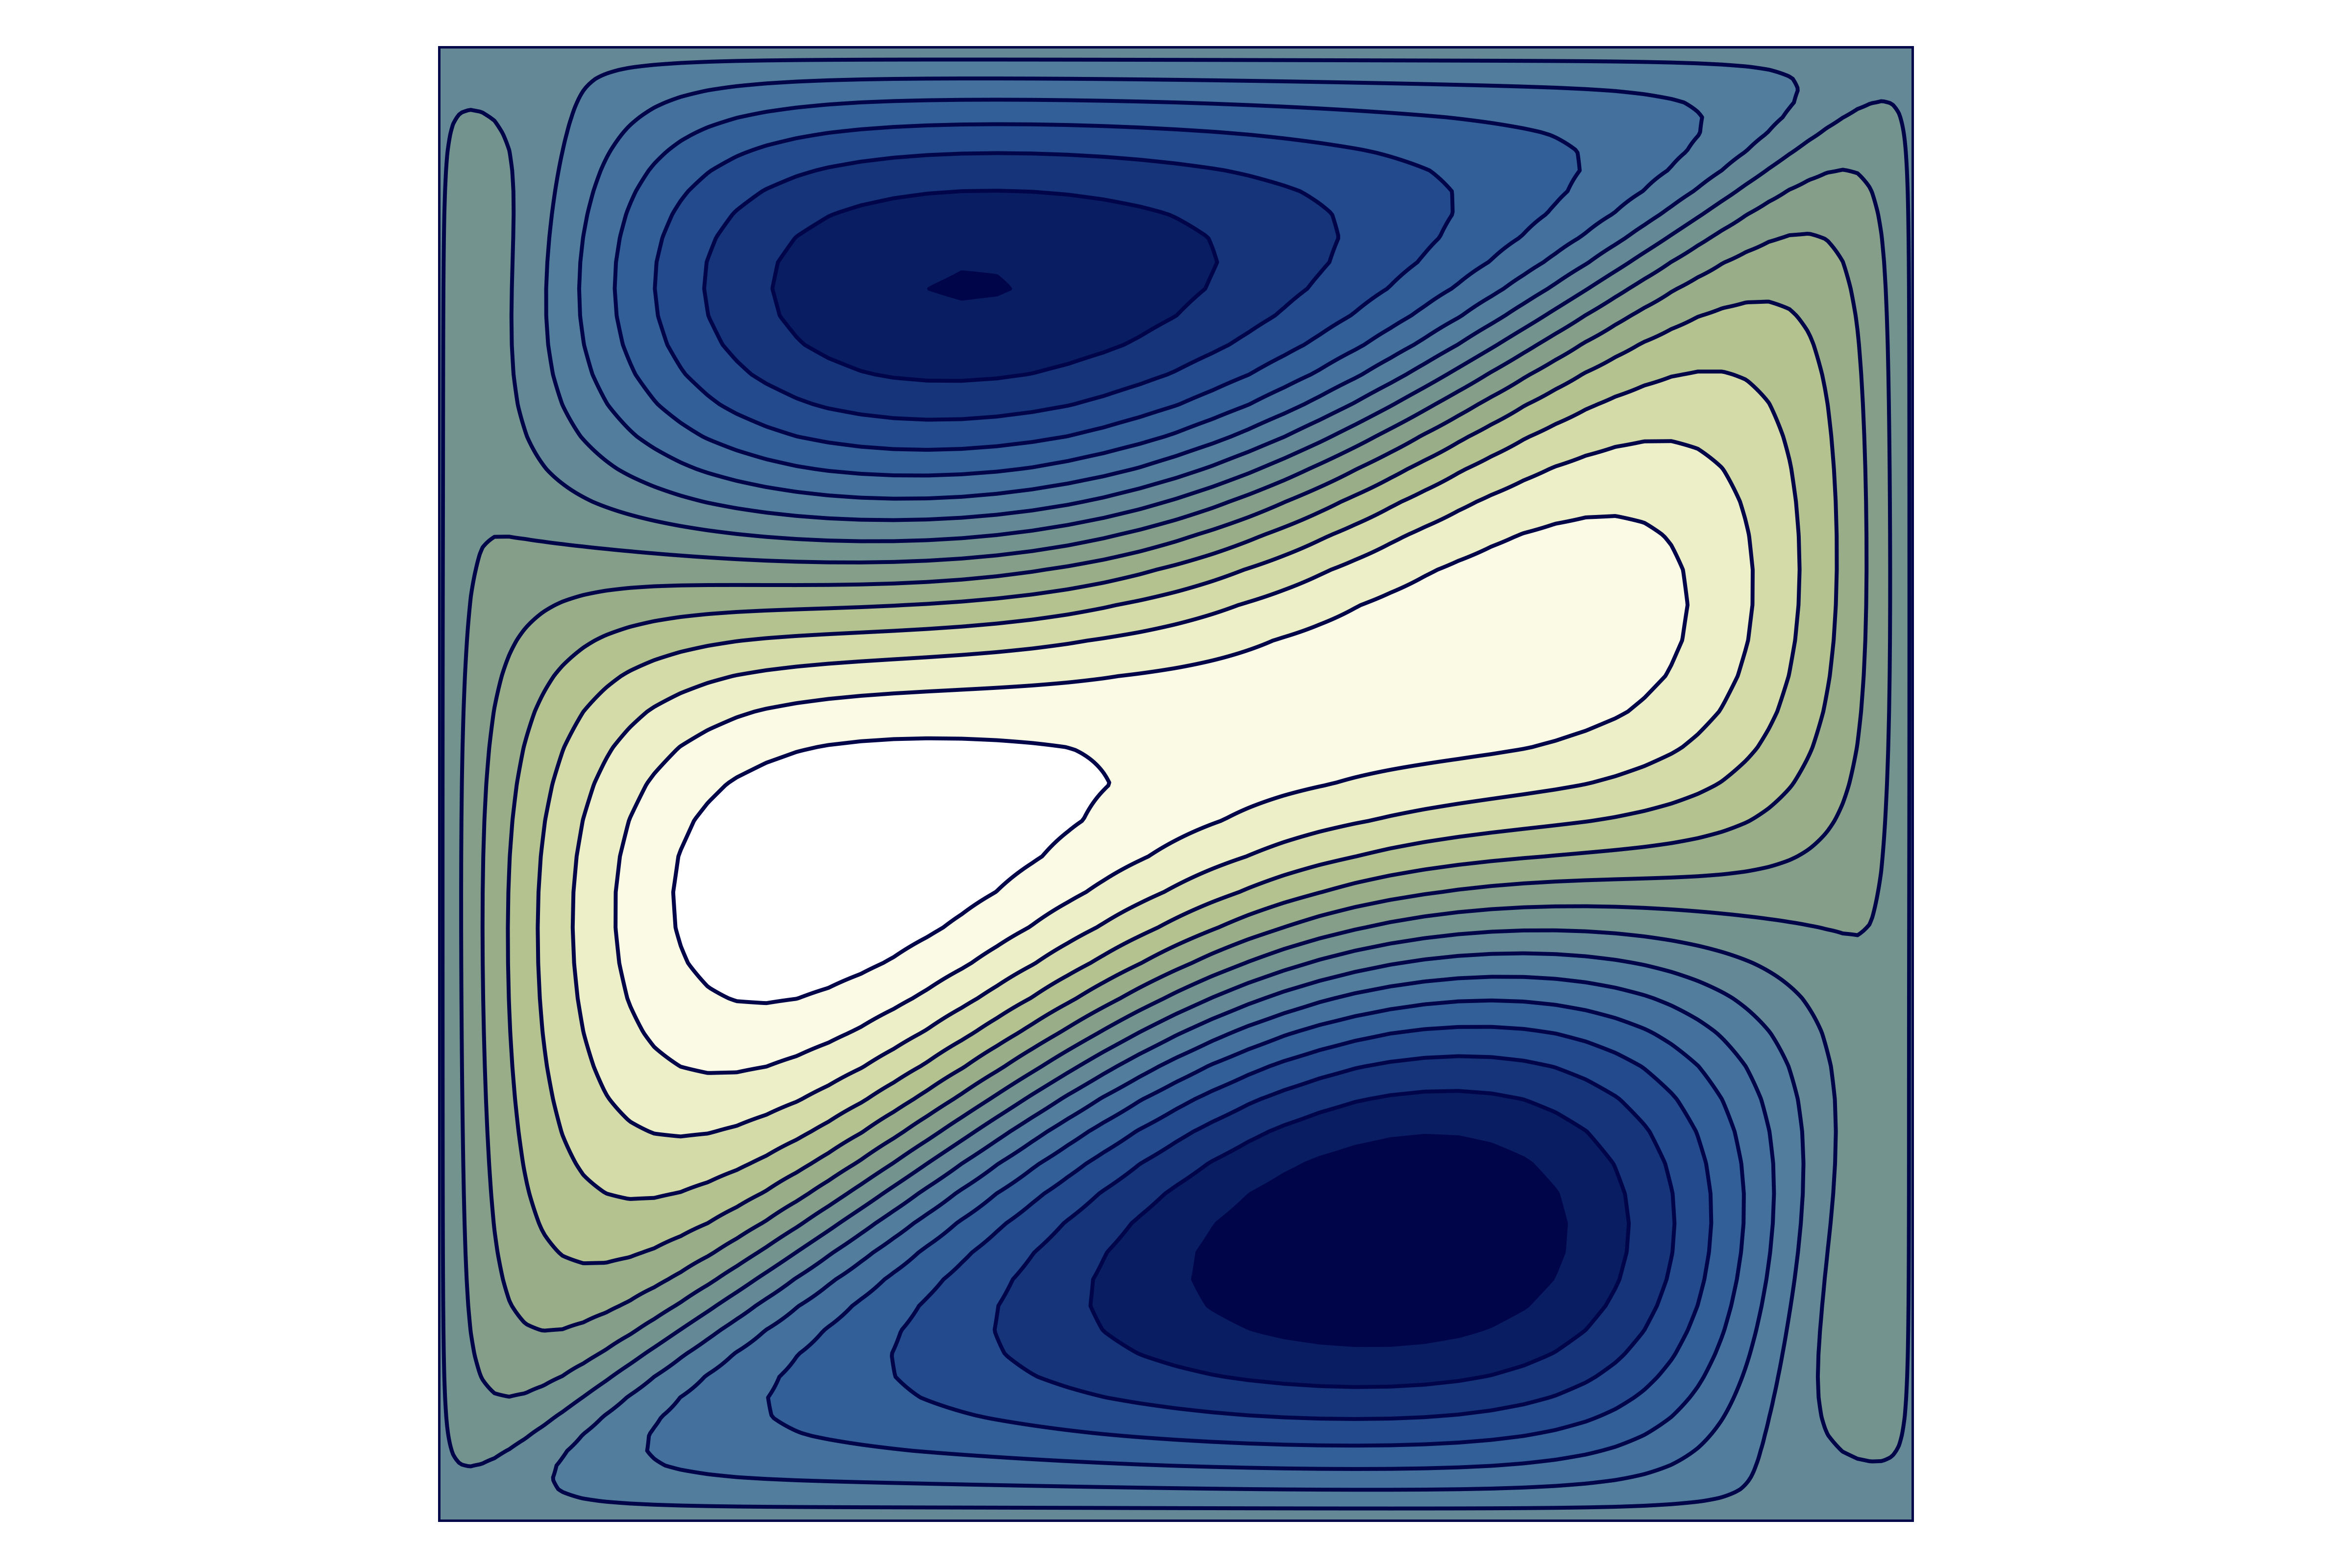
\includegraphics[width=\textwidth]{figs/psi_Re375.000_branch2_u_t_bigger.png}
\end{subfigure}
\caption{Streamlines for the pitchfork $P_3$ to the left and the two asymmetric
  solutions of the new branches to the right}
\label{fig:sol_branch2}
\end{figure}

\begin{figure}[h!]
  \centering
  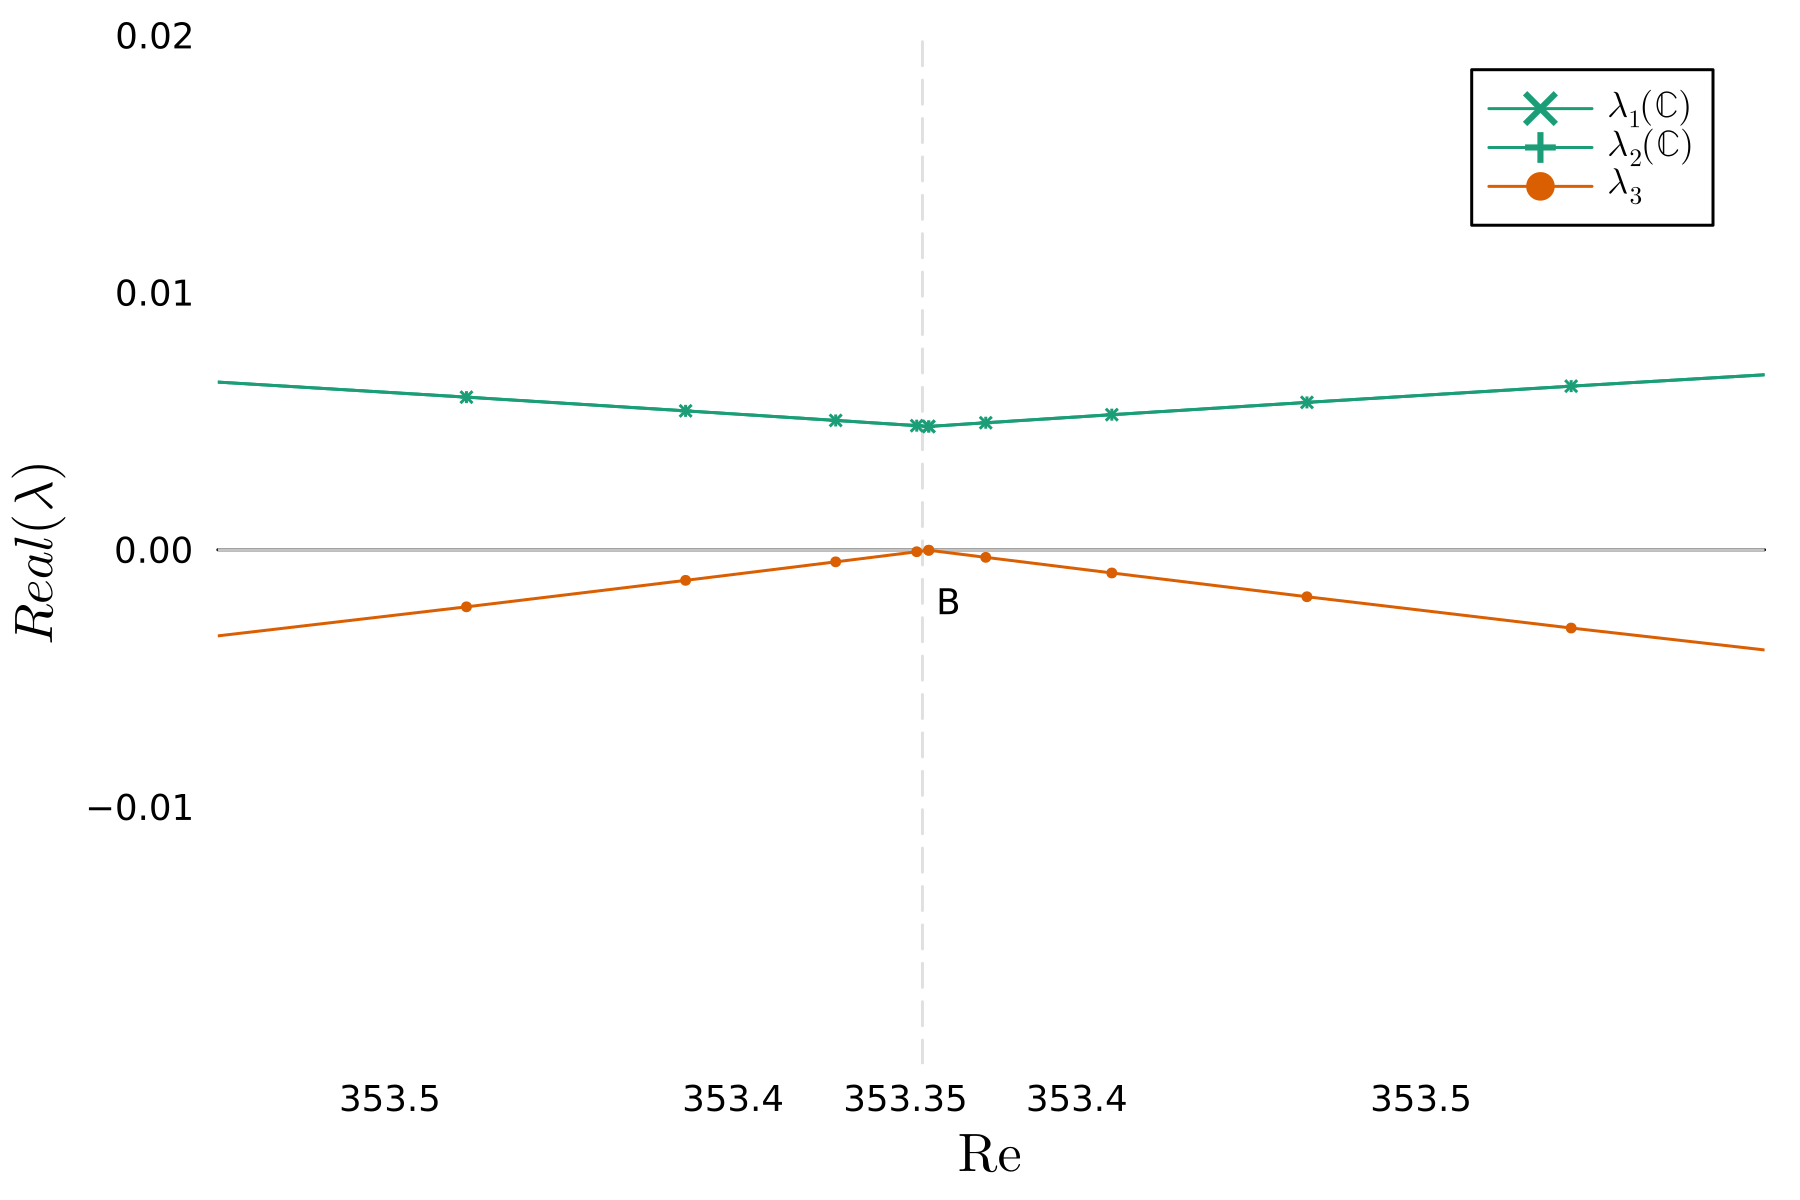
\includegraphics[width=0.7\textwidth]{figs/lsa_sn_branch2_zoom96x96.png}
  \caption{Linear stability analysis around connection $B$ of second branch
  (decreasing and then increasing Reynolds number), grid $96 \times 96$}
  \label{fig:lsa_branch2}
\end{figure}

The question which remains is what happens at the saddle-node at point $C$. The
schematic in figure \ref{fig:schem_saddle} shows the evolution of the
eigenvalues, and figure \ref{fig:lsa_zoom} shows a detail on real part of the
eigenvalues for figure \ref{fig:lsa}. After the Hopf bifurcation ($A$), we have
a complex conjugate pair with nonzero imaginary components and with a positive
real part. From pitchfork $P_3$ ($B$) onwards, the additional eigenvalue
$\lambda_3$ has a real part becomes also positive. What happens at the
saddle-node $C$ is, first of all, that the two eigenvalues lose their imaginary
part and become purely real. Moreover, this takes place at a nonzero real part.
What seems to be happening "simultaneously" or just after that is one of the
complex pairs (now real) jumps and becomes negative. The eigenvalue
configuration is depicted in the complex plane in figure \ref{fig:complexplane}
to illustrate the behavior. This phenomenon is speculative because we cannot be
sure that it is the eigenvalue corresponding to the complex pair that becomes
stable. It could be that two positive eigenvalues meet at the saddle-node.
Additionally, these interpretations must be taken cautiously as the saddle-node
is a highly degenerated point where the Jacobian is ill-conditioned. On top of
these unreliably converged points of the Newton solver, we are doing a linear
stability analysis. Due to the degeneracy it may even be that the saddle-node
is a double or triple zero, in terms of eigenvalue crossings. Nonetheless,
these results were obtained on a large grid for a pseudo-spectral code of size
$96 \times 96$.


\begin{figure}[h!]
  \centering
  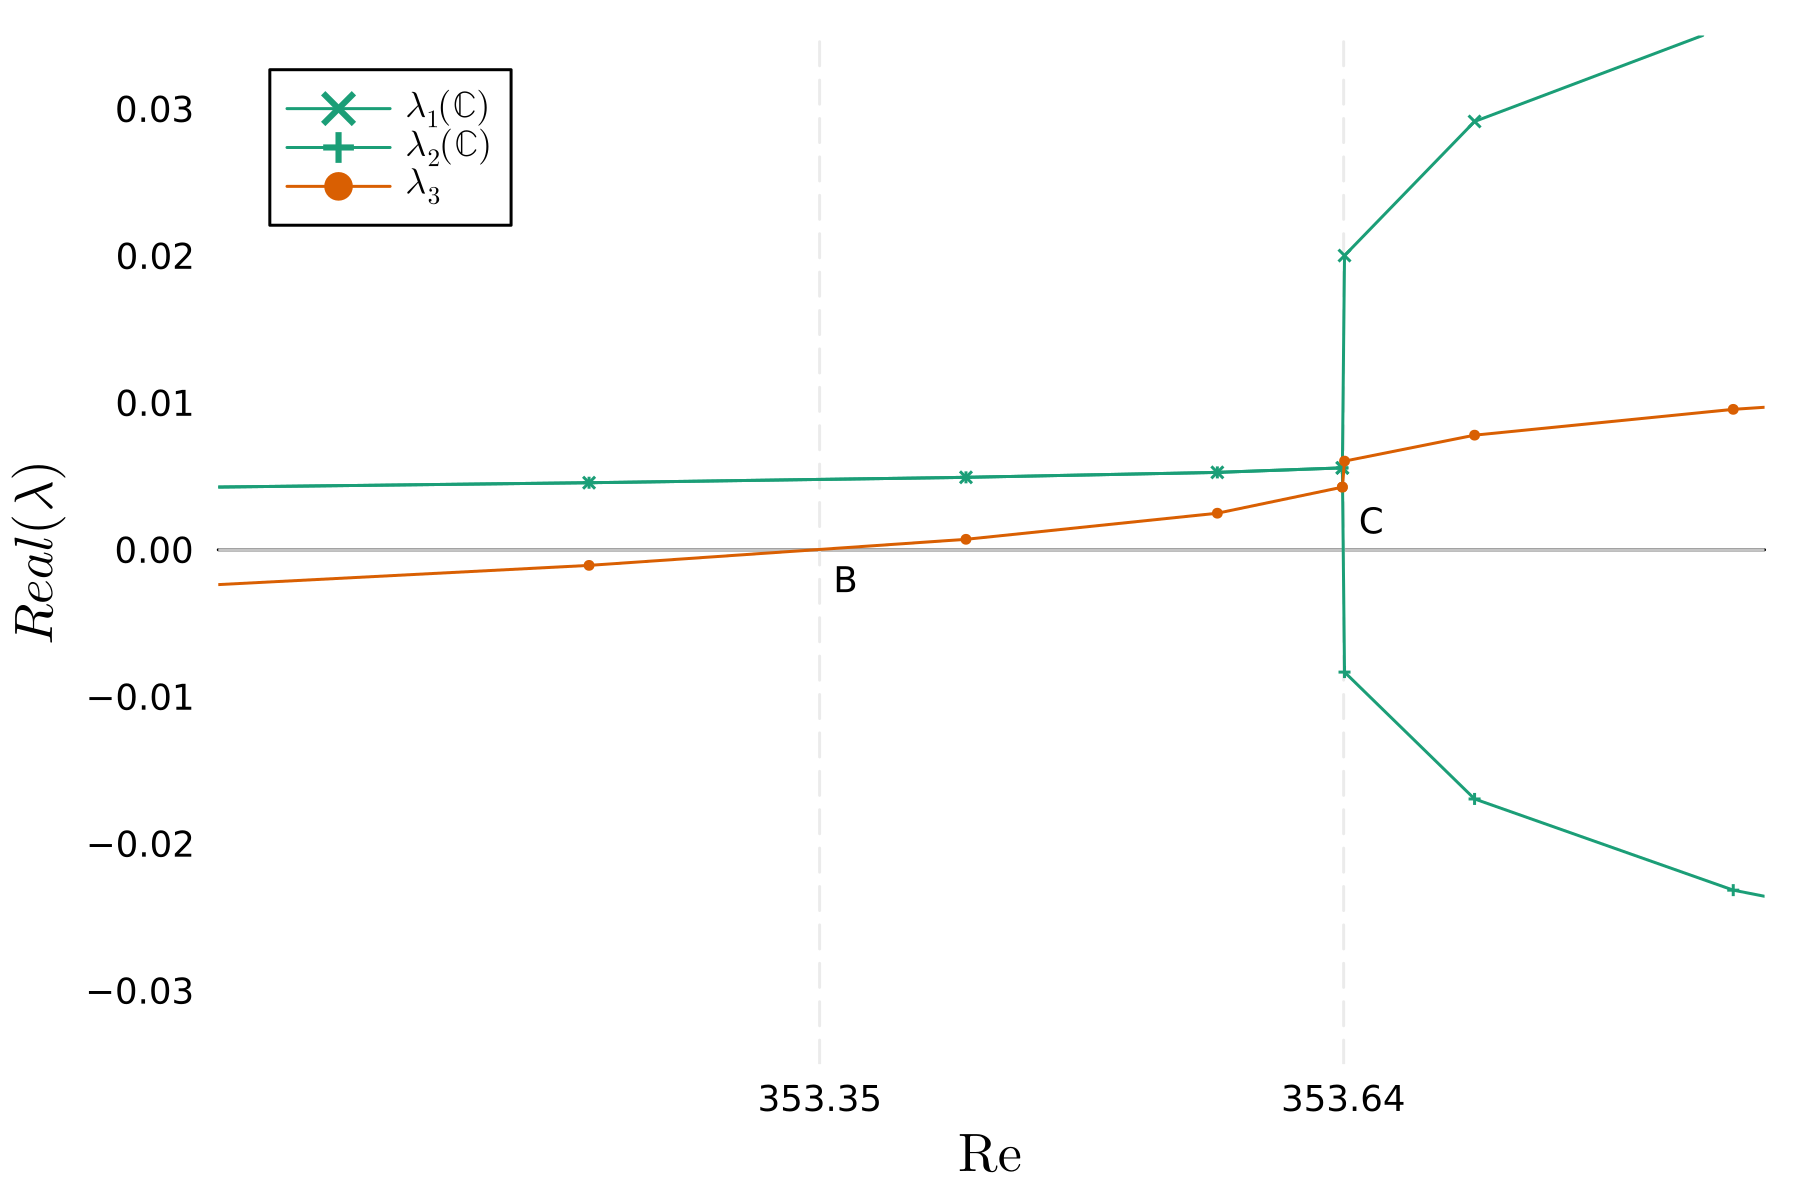
\includegraphics[width=0.6\textwidth]{figs/lsa_sn_zoom96x96.png}
  \caption{Zoom of figure \ref{fig:lsa} on location of saddle-node at Reynolds $353.654$} 
  \label{fig:lsa_zoom}
\end{figure}

\begin{figure}[h]
\centering
\begin{subfigure}[b]{0.3\textwidth}
  \centering
  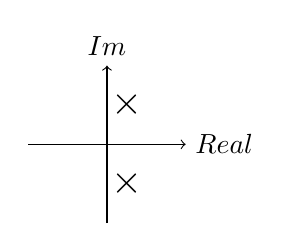
\begin{tikzpicture}
    \draw[->] (-1,0) -- (1,0) node[right] {$Real$};
    \draw[->] (0,-1) -- (0,1) node[above] {$Im$};
    \node at (0.25,0.5) {\textbf{\Large $\times$}};
    \node at (0.25,-0.5) {\textbf{\Large $\times$}};
  \end{tikzpicture}
  \caption{$1\mathbb{C}^+$, before saddle-node $C$ \newline}
\end{subfigure}
\begin{subfigure}[b]{0.3\textwidth}
  \centering
  \begin{tikzpicture}
    \draw[->] (-1,0) -- (1,0) node[right] {$Real$};
    \draw[->] (0,-1) -- (0,1) node[above] {$Im$};
    \node at (0.25,0) {\textbf{\Large $\times$}};
  \end{tikzpicture}
\caption{$2\mathbb{R}^+$, "just" before saddle-node $C$}
\end{subfigure}
\begin{subfigure}[b]{0.3\textwidth}
  \centering
  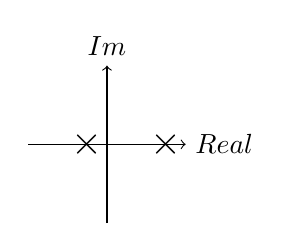
\begin{tikzpicture}
    \draw[->] (-1,0) -- (1,0) node[right] {$Real$};
    \draw[->] (0,-1) -- (0,1) node[above] {$Im$};
    \node at (0.75,0) {\textbf{\Large $\times$}};
    \node at (-0.25,0) {\textbf{\Large $\times$}};
  \end{tikzpicture}
\caption{$1\mathbb{R}^+$, at the saddle-node $C$ \newline}
\end{subfigure}
\caption{Visualization of the real and imaginary part of the complex conjugate pair
  $\lambda_1$ and $\lambda_2$ of figure \ref{fig:lsa} and \ref{fig:lsa_zoom}.}
\label{fig:complexplane}
\end{figure} 

\subsection{A useful Benchmark Problem?}

This problem was chosen with the primary intention to investigate it as a
potential benchmark to test Navier-Stokes solvers. We have seen that the
problem exhibits a wide variety of bifurcation scenarios. First, there is a
Hopf bifurcation, which is interesting because it shows if such periodic orbits
can accurately be detected using as a benchmark. Additionally, there is another
pitchfork $P_3$ close to the saddle-node. As mentioned, the Reynolds numbers
are very low, and the computational cost is not too high to compute such
solutions. Regularizing the boundary conditions for a given solver is
straightforward as well, and the square domain should be easily discretizable.
This makes up for a great benchmark. It just has to be clarified what exactly
happens at the saddle-node.

\subsection{Future Work}

This work provides an implementation of the four-sided cavity flow in Julia,
and the code can reproduce the original discontinuous problem. We have seen
that the problem involves more bifurcation scenarios than originally
anticipated. In the regularized version, there is the additional pitchfork
bifurcation and the Hopf bifurcation, which leads to stable periodic orbits.

The abovementioned more complicated crossing at the saddle-node needs further
refinement of the states of the continuation algorithm. An exact comparison to
the MATLAB code at high resolution would be required to clarify the issue. But
it seems that the Hopf bifurcation and pitchfork $P_3$ can be seen independent of
the problem arising at the saddle-node. 

Another option is related to the symmetries of the cavity. Using a square
cavity and having the four lid's velocities changing at the same time means
that we are varying 4 Reynolds numbers simultaneously. From a geometrical point
of view, that reflects that we are moving on a line in a four-dimensional space
of the four Reynolds numbers that could be varied. On this four-dimensional
line we have 

To get a better picture of what is happening, on can break the symmetries of
the problem and impose different Reynolds numbers at the lid. This could
separate the dense scenario of eigenvalues near the saddle-node.

Moreover, we have always worked with the regularized version to be sure of the
convergence rate for our pseudo-spectral discretization. It could be
interesting to see if one can reproduce the periodic orbits and the secondary
branch and compare the critical Reynolds numbers in the discontionuous case.
Conversely, \citet{chen2013} used a finite difference discretization. With the
pseudo-spectral approach, it is for sure not guaranteed to get a useful
approximation of the original boundary conditions. Another strategy
is trying the spectral approach on the un-regularized version and seeing how
the convergence rates and results are affected.

Lastly, it has to be mentioned that there is another eigenvalue crossing
happening close to the pitchfork $P_2$ at the unstable base solution. This was
not investigated in this study but could suggest a more complex picture of the
bifurcation scenario at $P_2$. Further, as already mentioned, $P_2$ only
connects unstable branches.

In terms of implementation, the Julia module could be further extended. For
now, the continuation algorithm and the linear stability analysis results are
saved in a CSV format, and the values of the streamfunctions at the grid points
are stored in plain text files. A further optimization could be to directly
save results as binaries in an HDF5 format. This could easily be done with a
package called \emph{JLD.jl} and would probably reduce the code size and
simplify the results handling. Another thing worse mentioning is that the code
is divided into the core functions explained in the section \ref{sec:impl} on
the code necessary to run the simulations and generate the plots. For
simplicity, the Julia module only includes the core functions presented in
section \ref{sec:impl}. It could be beneficial to have both parts reconciled,
and the binary savings of results would greatly help.

